\chapter{Introduction}
The recent discovery of a Higgs boson at the \ac{LHC} \cite{Aad:2012tfa} with properties in agreement with those predicted by the \ac{SM}, leaves the particle physics community in the situation where there is no definitive course of action through which new physics might be discovered. As a result there are two main ways in which we can proceed-- we can continue to push forward in the ``energy frontier'' (as is currently being done at the \ac{LHC}) and look for new particles not predicted by the \ac{SM} but by other compatible models such as supersymmetry, or we can push forward in the ``precision frontier'' (e.g. by making detailed measurements of boson decays) to reduce the uncertainty on our current measurements until we see a deviation from the \ac{SM} predictions. Both approaches have their benefits and drawbacks but have the possibility of discovering new physics.

Pushing the energy frontier has the advantage that most popular \ac{BSM} theories predict particles at higher energy than we have currently explored and so there is a strong chance that if we continue to increase the centre of mass energy of collisions we will eventually see something new. It also has the obvious advantage that we already have a collider that is doing this type of exploration, namely the \ac{LHC}. That being said, most \ac{BSM} theories have very loose constraints on the absolute mass of these undiscovered particles (in some models \cite{Baer:2012uy} they are ${>}$1TeV) and so it is possible that the collision energy needed to discover them is either unaffordable or technically unfeasible with our current level of technology. As such, even if we invested a considerable amount of money and pushed accelerator technologies to their limit we might still see nothing new.

Pushing the precision frontier has the drawback that there is no guarantee that it will do anything but reinforce our belief in the \ac{SM}. However we know that constraining the parameters of the \ac{SM} may allow us to exclude many current \ac{BSM} theories and to constrain future predictions. It also has the benefit that there is the possibility of infering the presence of new particles at lower energies that were missed in hadron colliders where there were too many background events to distinguish signal events. 

In practice the best solution will be to use both approaches in parallel. Here we will look at two potential future colliders (The \ac{ILC} and \ac{CLIC}) that are focused on high precision physics but which act at sufficiently high energy that they may be capable of discovering new particles themselves, or at least characterising any new particles discovered at the \ac{LHC}. 

\chapter{Physics Justification For A Linear Lepton Collider}
\section{Benefits Of Using Leptons}
\label{benefits}
The \ac{ILC} and \ac{CLIC} are the two most developed designs for a future high precision device. In both cases the main method for achieving the high level of precision is to use leptons (specifically electrons and positrons) as the colliding particles. The main benefit of using leptons over hadrons is that it dramatically reduces the level of uncertainty in the initial conditions of the collisions. Using two fundamental particles means that there is little uncertainty on the initial energy of the system as the collision is simply an annihilation process with no parton energy distribution to consider (as is the case for hadron colliders.) This means that the initial energy for any collision is known to simply be the sum of the two beam energies and so the entire uncertainty in the initial conditions can be attributed to uncertainties in the beam properties. These uncertainties are caused by processes such as Bhabha Scattering (\reffig{Fig:Bhabha}) and Bremsstrahlung (a form of synchotron radiation) which result in the scattering of the beam particles either through photon emission/exchange, or through the annihilation of an electron positron pair into a photon (or Z Boson) which then produces a new electron positron pair with different momenta. These processes are collectively referred to as \ac{ISR}. In the case of a photon being emitted by the beam, the photon will sometimes decay into quark-antiquark pairs if it carries enough energy causing hadronic contamination of the beam. Because these processes are the main source of uncertainty in the collision, considerable work has been done to reduce them by altering the beam structure used in the colliders and developing advanced beam-monitoring technology. As a result the beam energy distribution is now expected to be known to a precision of ${10^{-4}}$ \cite{2009JInst...410015B} at \ac{ILC}.  The beam energy distribution at \ac{CLIC} is expected to be slightly worse due to differences in the beam structure used but it is still small when compared to the parton energy distribution at a hadron collider. Another major benefit of a lepton collider is that, because the initial energy of the collision is known to a high accuracy, the beam energy can be tuned to a particular resonance which strongly favours the production of a certain particle allowing us to choose what processes we want to look at.
\begin{figure}
  \centering
    \subfloat[]{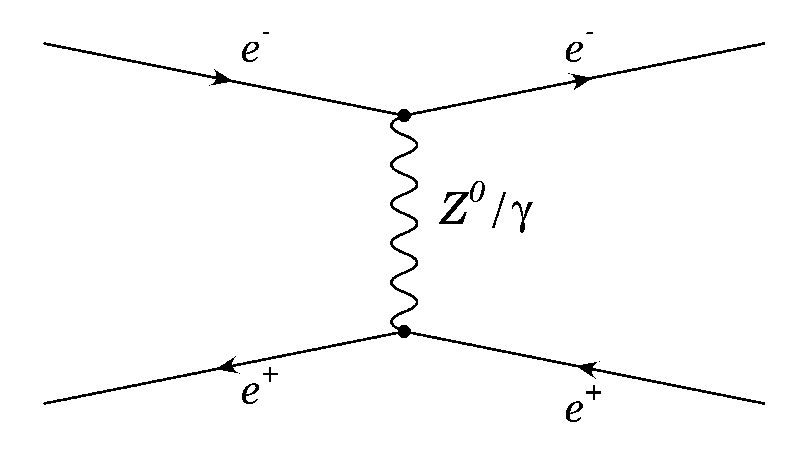
\includegraphics[width=0.48\textwidth,height=5cm,keepaspectratio]{fig/bhabha-t.png}}
    \subfloat[]{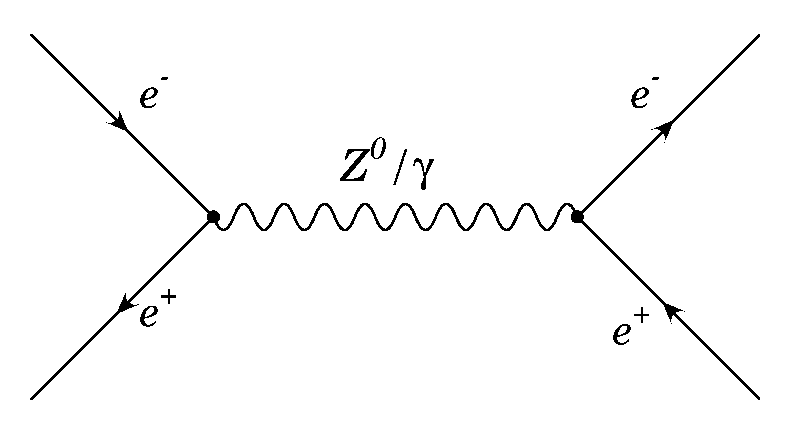
\includegraphics[width=0.48\textwidth,height=5cm,keepaspectratio]{fig/bhabha-s.png}}
  \caption[ISR Processes For An Electron Positron Collider]{Bhabha scattering processes in which the electrons and positrons exchange a photon (t-channel, left) or annihilate and reform (s-channel, right) resulting in a change of energy, momentum and direction of motion of the particles.}
  \label{Fig:Bhabha}
\end{figure}
While leptons greatly improve the potential precision of any measurements we could make, they are somewhat problematic to accelerate efficiently. Ideally in any accelerator we would like to accelerate the particles in a ring so that we can continuously accelerate the particles for long times in a relatively compact space. However for electrons this is not possible due to synchrotron radiation- the energy lost when a charged body is accelerated through a magnetic field. The rate of energy loss due to synchotron radiation is given by \refeq{Eq:synchotron radiation}:
\begin{equation}
\label{Eq:synchotron radiation}
P = \frac{e^4}{6\pi\varepsilon_0m^4c^5}E^2B^2.
\end{equation}
Where $e$ is elementary charge, $E$ is particle energy, $B$ is magnetic field, $m$ is mass and all other symbols have their usual meaning.

Because the power is dependent on the inverse mass of the particle to the fourth power, this means that the energy lost for an electron is of the order ${10^{12}}$ times greater than for an equivalent proton undergoing the same acceleration. This makes it unfeasible to accelerate electrons to energies comparable to the scale of the \ac{LHC} using a circular collider.

One obvious solution would be to use muons rather than electrons due to their significantly higher mass. However, this has its own problem in that muons only exist for 2.2${\mu}$s before decaying and so need to be accelerated and collided within a very narrow time frame. As a result the more practical solution is simply to build a linear collider with a large accelerating gradient instead.

While this does limit the maximum feasible energy (as a higher energy would require a longer accelerator which would be more expensive and restricts the locations in which a collider might be built) it is worth remembering that unlike in hadron colliders, lepton colliders use the full beam energy as they collide fundamental rather than composite particles and so a lower beam energy lepton collider can still have similar discovery potential to a higher energy hadron collider.

\section{Higgs Production In An Electron-Positron Collider}
The main aim for any future linear lepton collider will be to measure the mass, cross-section and couplings of the Higgs Boson as these are accurately predicted by the \ac{SM} but in many cases the experimental uncertainties are still relatively large. As such it is useful to look at the ways in which a Higgs might be produced in an electron positron collision. The cross sections for the various production methods are shown in \reffig{Fig:HiggsCrossSections} but in practice there are three dominant production methods: Higgsstrahlung, WW fusion and ZZ fusion which are shown in more in detail in \reffig{Fig:WWFusion}, \reffig{Fig:ZZFusion} and \reffig{Fig:HiggsStrahlung}. The WW and ZZ fusion processes are collectively known as \ac{VBF} and are the dominant production methods for energies ${>}$500GeV while Higgsstrahlung dominates at lower energies.
\begin{figure}
  \centering
  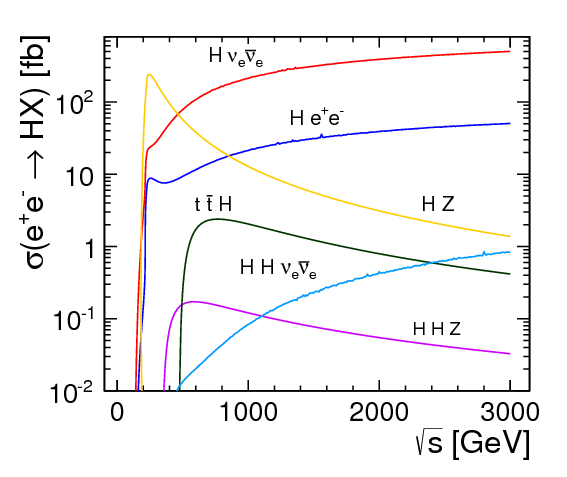
\includegraphics[width=0.75\textwidth,height=10cm,keepaspectratio]{fig/HiggsCrossSections}
  \caption[Higgs Cross Sections]{Cross sections for Higgs production mechanisms in an ${e^+e^-}$ collider as a function of centre of mass energy. The main processes of note are WW Fusion(red), ZZ Fusion(blue) and Higgsstrahlung(yellow.) Image taken from \cite{Simon:2014aqa}. }
  \label{Fig:HiggsCrossSections}
\end{figure}

\subsection{WW Fusion}
\begin{figure}[h]
  \centering
  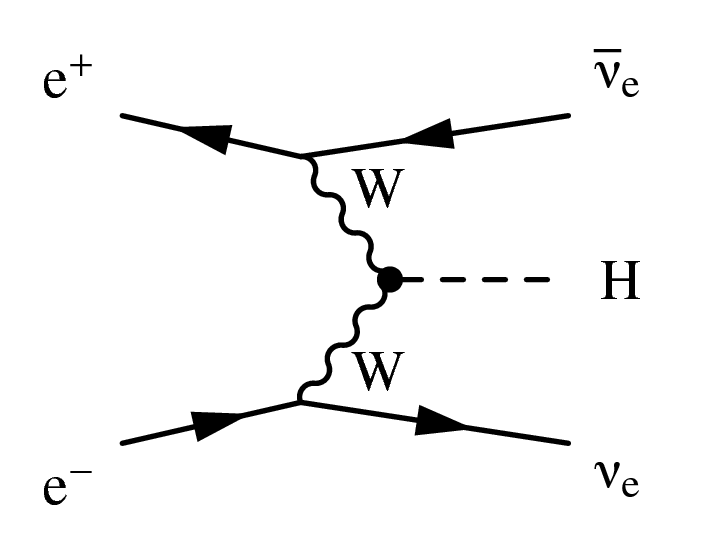
\includegraphics[width=0.75\textwidth,height=5cm,keepaspectratio]{fig/WWFusion}
  \caption[WW Fusion]{Production of a Higgs Boson in association with two neutrinos via fusion of two W Bosons. Image from \cite{Simon:2014aqa}.}
    \label{Fig:WWFusion}
\end{figure}

WW fusion will be the dominant Higgs Production mechanism at any high energy lepton collider due to its high cross-section. While the fact the Higgs is produced in association with two high energy neutrinos limits our ability to use our precise knowledge of the initial state of the collision it is also beneficial as it means we will produce very clean signals in which any particle seen by the detector can be assumed to have come from the Higgs decay.
\subsection{ZZ Fusion}
\begin{figure}[h]
  \centering
  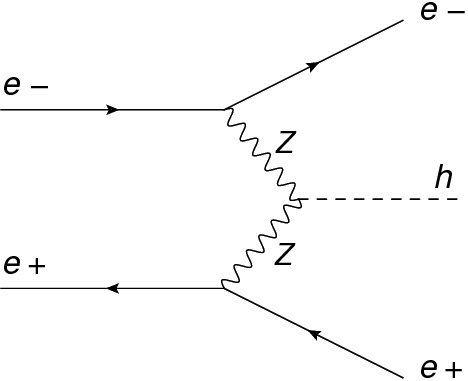
\includegraphics[width=0.75\textwidth,height=5cm,keepaspectratio]{fig/ZZFusion}
  \caption[ZZ Fusion]{Production of a Higgs Boson in association with an electron-positron pair via fusion of two Z Bosons. Image from \cite{Han:2015ofa}.}
  \label{Fig:ZZFusion}
\end{figure}

ZZ fusion is the second most dominant process for a lepton collider. Unlike the WW fusion process, here we have no missing energy due to neutrinos and so we can use our knowledge of the initial state to put restrictions on our measurements of the Higgs. However, the electron and positron produced in association with the Higgs will often be highly boosted and so will sometimes stay very close to the beam axis and escape the system without being detected, so it is still possible that we can lose our knowledge of the initial state. 
\subsection{Higgsstrahlung}
\begin{figure}[h]
  \centering
  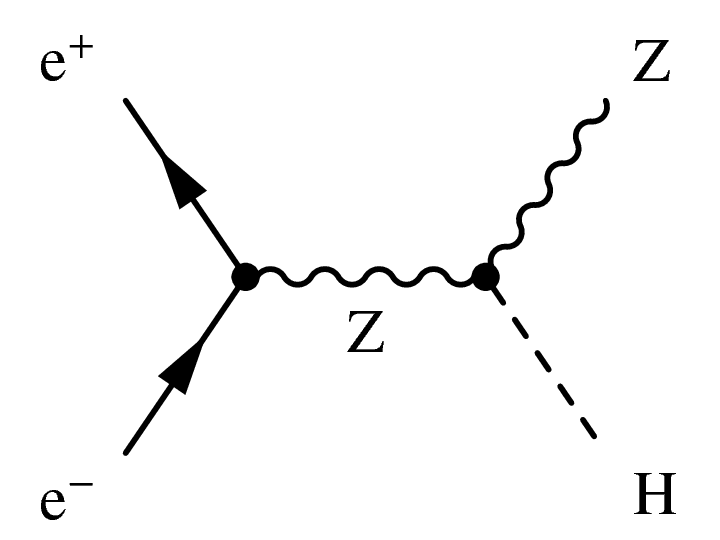
\includegraphics[width=0.75\textwidth,height=5cm,keepaspectratio]{fig/HiggsStrahlung}
  \caption[Higgsstrahlung Process]{Production of a Higgs Boson in association with a Z Boson. The Z Boson is produced directly through annihilation of an  electron with a positron then radiates the Higgs Boson. Image from \cite{Simon:2014aqa}.}
  \label{Fig:Higgsstrahlung}
\end{figure}

While the Higgsstrahlung process is only dominant at lower energies it is often referred to as the “Golden Higgs Production Mode” as it allows for model-independent measurements of the Higgs, something that cannot be done at other colliders. This is because in cases where the Z decays to easily reconstructable particles such as a pair of high energy muons, because we know the initial state energy with high precision, we are able to calculate the properties of the Higgs without actually looking at its decay products. This means we do not need to make any assumptions about the decay modes of the Higgs and the efficiency with which they are observed, and so the results are independent of our model for the possible Higgs interactions. Through this process we can make precise measurements of the Higgs mass from the recoil against the Z, the total Higgs cross section and the coupling of the Higgs to the Z Boson.

By using measurements from the Higgsstrahlung production mechanism combined with direct measurements of the various different Higgs decay modes it will be possible to calculate many of the properties of the Higgs (cross-section, coupling strengths etc) to the unprecedented level of ${<}$1\% uncertainty. If new physics processes are not present below $\sim$1TeV then the expected deviations of the Higgs couplings are expected to be of the order 1-10\% and so this high level of precision is essential for verifying \ac{BSM} models \cite{PhilBurrows}. The \ac{LHC} is only expected to be able to measure the necessary Higgs couplings to the order 1-10\% precision and so lacks the resolution to make definitive tests of many \ac{BSM} models at this scale. If no direct evidence for new physics processes is seen at the 1TeV scale in the \ac{LHC} (e.g.\ by discovering a new particle) then the \ac{ILC} may still be sensitive to them through precision measurements. The precision of the Higgs couplings predicted for the \ac{ILC} and a comparison to those achievable by the \ac{LHC} can be seen in \reffig{Fig:HiggsCouplings} and \reffig{Fig:LHCvsILC}.  
\begin{figure}
  \centering
  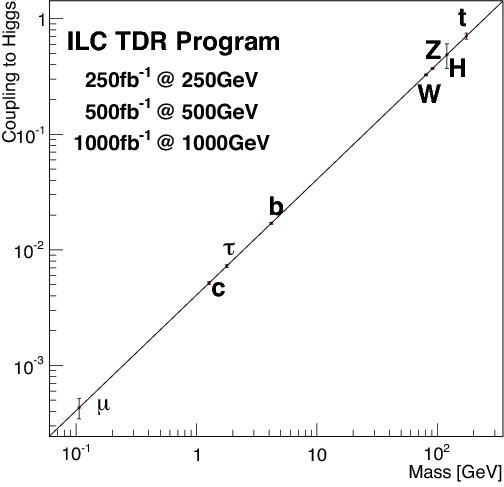
\includegraphics[width=0.75\textwidth,height=10cm,keepaspectratio]{fig/HiggsCouplings2}
  \caption[Higgs Couplings]{Coupling strength of fermions and bosons to the Higgs Boson as a function of their mass. The uncertainities shown are for the full \ac{ILC} run and assume the \ac{SM} predictions for the couplings are correct. Taken from \cite{Fujii:2015jha}}
  \label{Fig:HiggsCouplings}
\end{figure}

\begin{figure}
  \centering
  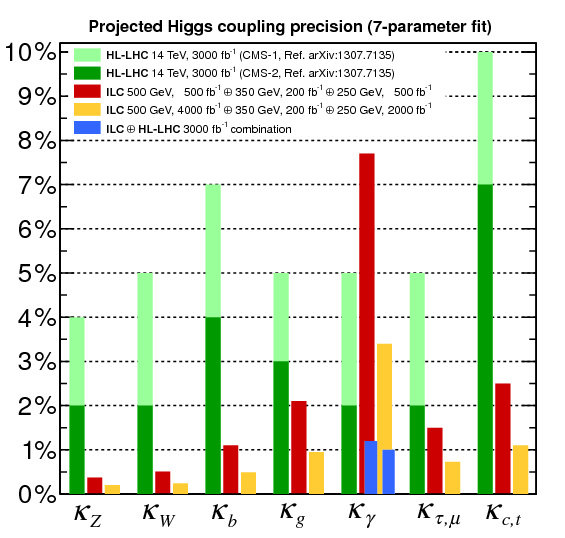
\includegraphics[width=0.75\textwidth,height=10cm,keepaspectratio]{fig/LHCvsILC}
  \caption[Predicted Relative Coupling Precision For ILC vs LHC]{Predicted relative precision of Higgs Couplings when measured at the ILC compared to the LHC. The energy staging referenced here for the ILC varies slightly from that mentioned in the ILC technical design report \cite{ILCTDR} running scheme though the overall result is still expected to be similar. Taken from \cite{Fujii:2015jha}}
  \label{Fig:LHCvsILC}
\end{figure}

\chapter{Proposed Experiments}
There are many possible designs for future lepton colliders \cite{Lipton:2012du,Koratzinos:2014cla} however here we will focus on the two most developed projects, \ac{CLIC} and \ac{ILC}. Both projects propose using electron-positron collisions and were founded over twenty years ago though \ac{ILC} is currently the more mature design of the two. We will also discuss the detectors proposed for both experiments, the \ac{ILD} and the \ac{SiD}. Both of these detectors were originally designed for use at \ac{ILC} as general purpose devices but are currently being adapted for use at \ac{CLIC}. Because the optimization of the detectors for use in \ac{CLIC} has only recently begun, the designs for both versions of the detectors are still similar enough that we will neglect describing both here but will instead describe just the \ac{ILC} versions of both detectors.

\section{ILC}

The ILC (\reffig{Fig:ILC}) is a proposed experiment consisting of a 31km ${e^+e^-}$ collider to be built in Kitakami in the northern region of Japan. The current construction schedule predicts the experiment will be finished in the mid-2020s with a cost of the order \pounds6 billion and will run for approximately 20 years. However, until funding is secured for the experiment this is just an estimate. The \ac{ILC} \ac{TDR} \cite{ILCTDR} was released in 2013 and gives a full description of the experiments' baseline design. While the \ac{TDR} is highly detailed, because the experiment is still under development it is possible that some of the information contained within it will become outdated and is likely to change in the future. For simplicity any figures given in this section can be assumed to be taken from the \ac{TDR} unless otherwise stated.

\begin{figure}
  \centering
  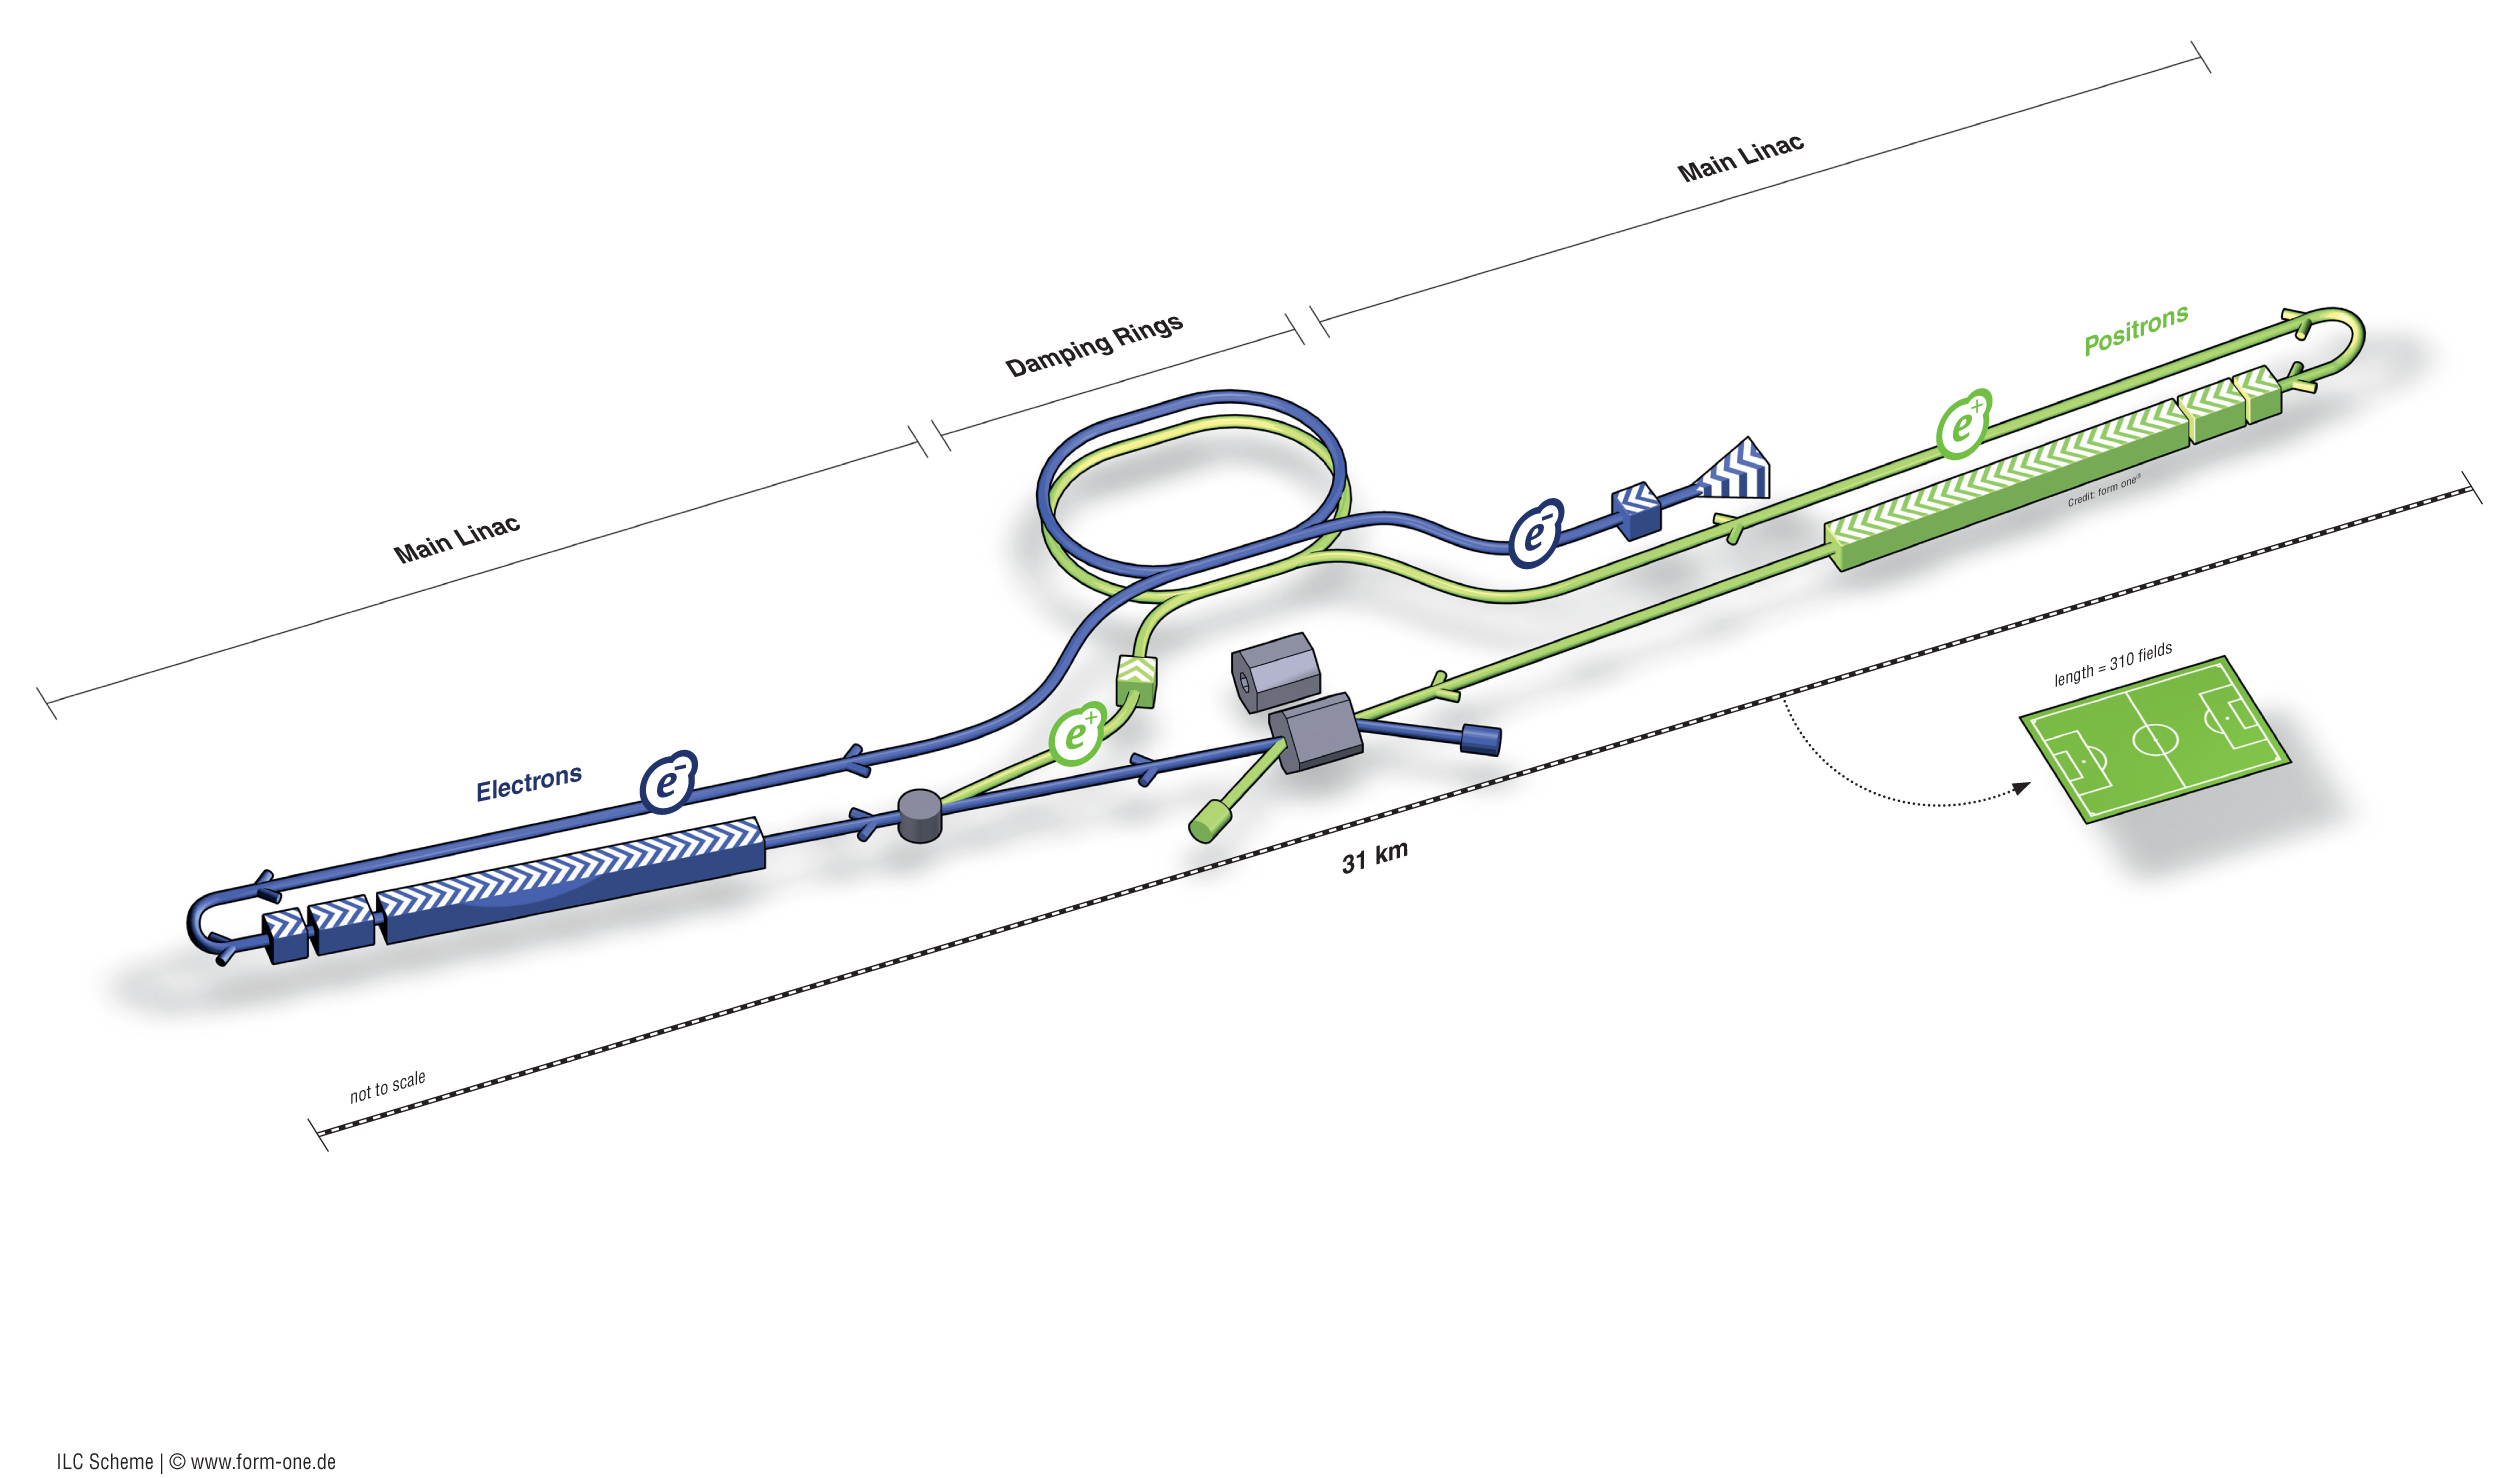
\includegraphics[width=0.75\textwidth,height=10cm,keepaspectratio]{fig/ILC}
  \caption[The ILC Experiment]{The \ac{ILC} Collider (from \cite{ILCTDR})}
  \label{Fig:ILC}
\end{figure}
\subsection{Energy Staging}
The \ac{ILC} will first be built with a maximum collision energy capability of 500GeV but with the potential for a later upgrade to 1TeV which would require doubling the length of the machine to 62km. The decision of whether the 1TeV upgrade is necessary will largely be determined by the results of the \ac{LHC} experiment; if any new particles are discovered above 500GeV then the 1TeV upgrade will be essential to characterise them. Assuming the 1TeV upgrade is realised the energy staging will be as described below.

The first three years will involve the ILC running at energy of 250GeV and taking 250fb${^{-1}}$ of data. The main aim at this stage will be to measure the Higgs mass and ZH cross section from the Higgsstrahlung process described above. At this energy the experiment will have little sensitivity to the Higgs-WW coupling.

For the following three years, the collider will run at 500GeV and will accrue 500fb${^{-1}}$ of data. The main aims here will be to measure the H-WW coupling, the total Higgs width and the absolute Higgs couplings to fermions. At this energy, measurements of top physics will also be possible including the top Yukawa coupling. Outside of the Higgs, the top quark is perhaps the least well measured of the standard model particles and so provides another area in which to look for deviations from the standard model predictions.

After this there will be the upgrade to 1TeV followed by another three years of running accumulating 1000fb${^{-1}}$ of data. The aim of running at this high energy will be to search for new particles such as dark matter candidates and supersymmetric particles. If one of these (or something entirely new) has already been discovered at the \ac{LHC} then the choice of 1TeV might be scaled down to somewhere between 500GeV and 1TeV to match the mass of the newly discovered particle.

After this the collider will undergo a high luminosity upgrade and will run at the same energies for the same time periods for another 9 years but instead accruing 900, 1100 and 1500${fb^{-1}}$ at the respective energies. This will allow for a further increase in the precision of all measurements taken during the lower luminosity run.
While the \ac{TDR} proposes the above run scheme for the \ac{ILC} there is still debate about what energies should be used with arguments being made for running at 90GeV (the Z mass) to gain precision measurements of the Z boson and 350GeV (the top production threshold) to better measure the properties of the top quark.

\subsection{Beam Production, Acceleration and Focusing}
\label{ILC:BEAM}

\begin{figure}
  \centering
  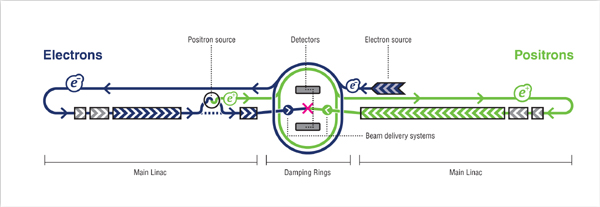
\includegraphics[width=0.75\textwidth,height=10cm,keepaspectratio]{fig/ILC_Simplified}
  \caption[Schematic Of The ILC]{A simplified schematic of the ILC}
  \label{Fig:ILCsimple}
\end{figure}

A simplified schematic of the \ac{ILC} accelerating structure is shown above in diagram \reffig{Fig:ILCsimple}. The first stage of the acceleration process is the production of electrons. This is done using the photoelectric effect by firing photons onto a GaAs target to produce photoelectrons. These electrons then enter a 3.2km long damping ring which accelerates the beam up to 15GeV. The primary purpose of the damping ring is to produce a homogeneous beam of electrons with uniform energy and momentum. After the damping ring the electrons enter into a two stage bunch compressor which separates the electron beam into ${\sim}$1300 bunches, each containing ${2\times10^{10}}$ electrons, with each bunch being separated by 554ns giving a beam pulse length of 730${\mu}$s. The overall intended collision rate of these pulses is 5Hz, which means that the duration for collisions is less than 1\% of the collision rate. This has important consequences for the detector design as it means the detectors have a large period of time in which to relax after events.As the detectors do not need to be on for 99\% of the time, it is considerably easier to cool them meaning the material budget for the cooling systems within them can be greatly reduced. Following the bunch compression the electrons enter the main 11km linac where they are accelerated up to the nominal beam energy using 7,400 1.3GHz superconducting niobium \ac{RF} cavities (see \reffig{Fig:cavity}) 

\begin{figure}
  \centering
  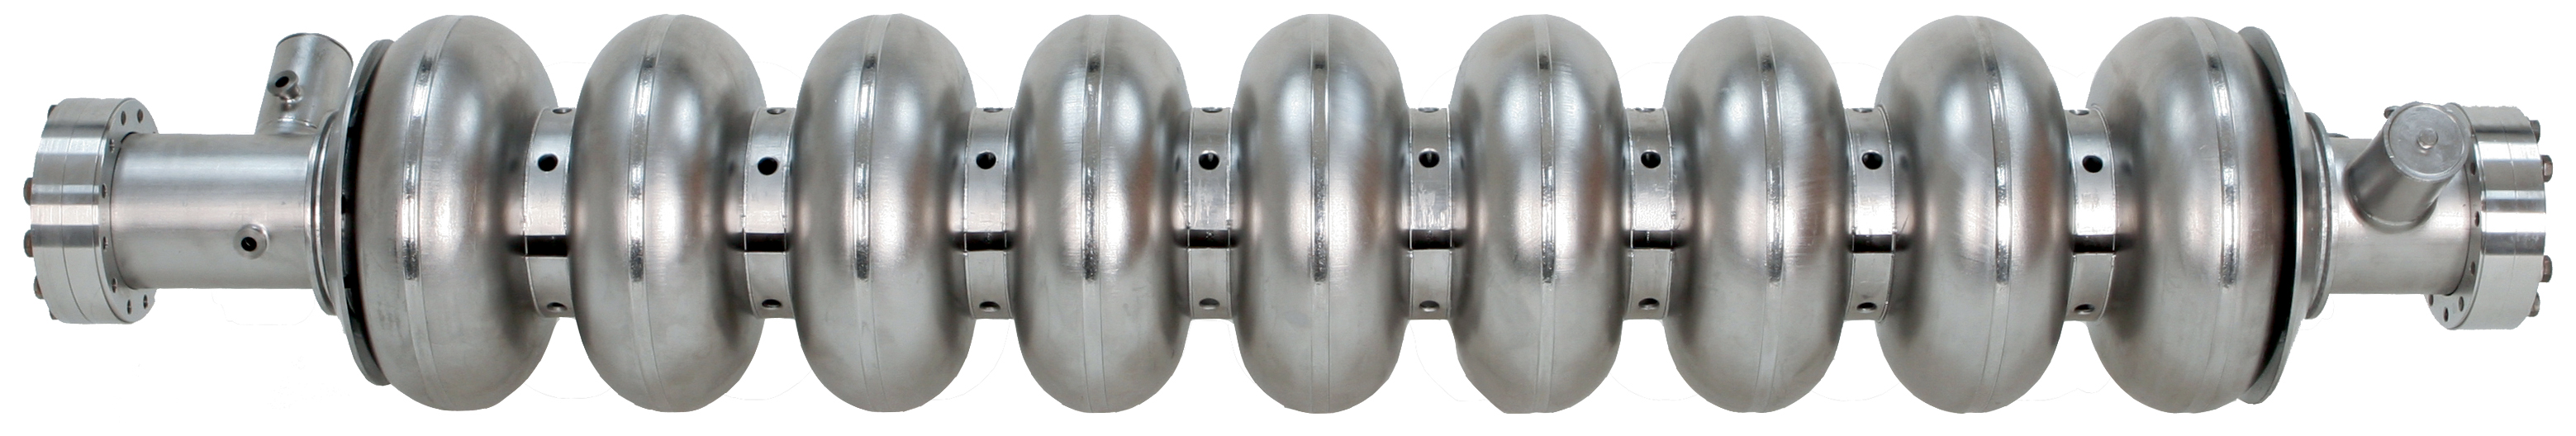
\includegraphics[width=0.75\textwidth,height=10cm,keepaspectratio]{fig/Cavity}
  \caption[Superconducting Cavities For The ILC]{A 1.3GHz Superconducting Niobium Radio Frequency Cavity \cite{ILCTDR}}
  \label{Fig:cavity}
\end{figure}
The \ac{RF} cavities are kept at a temperature of 2K and act to produce an average accelerating gradient of up to 31.5MV/m (14.7MV/m for the 250GeV stage.)  The final stage before the collision is the \ac{BDS} which primarily acts to compress the beam into a ribbon shape with a cross-section of 7.7 x 729.0 nm while also handling the beam monitoring. The ribbon shape acts to reduce the \ac{ISR} radiation described earlier (see \refsec{benefits}) while giving a small enough cross-section that the \ac{IP} of the collision can be well known. Following the \ac{BDS} the beam finally enters the detector and collides with the positron beam at a crossing angle of 14mrad then exits into the beam dump system which quenches what is left of the beam.
\subsection{Positron Production}
Positrons are produced at the \ac{ILC} by tapping off energy from the electron beam after it has been accelerated by the main linac. The electron beam is passed through an 'undulator' which causes the electrons to emit synchrotron radiation in the form of 10-30MeV photons by forcing the beam to take a rapidly varying path in the transverse plane. The resulting photons are then separated from the electron beam and are collided with a Titanium alloy target to produce electron positron pairs. The electrons and positrons are then separated- the electrons are dumped while the positrons are then passed into a damping ring and undergo all the same stages of acceleration and shaping as the electrons underwent before arriving at the \ac{IP}.
\section{CLIC}
\begin{figure}
  \centering
  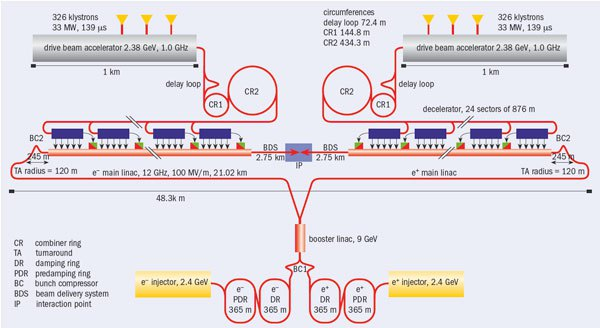
\includegraphics[width=0.75\textwidth,height=10cm,keepaspectratio]{fig/clic}
  \caption[The CLIC Experiment]{The CLIC Collider. Image taken from CLIC Conceptual Desgin Report\cite{CDR}}
  \label{Fig:CLIC}
\end{figure}
\ac{CLIC} is an experiment based at CERN which proposes the building of a 42km accelerator at the main CERN site in Geneva (\reffig{Fig:CLIC}.) Despite being named as “compact”, \ac{CLIC} is actually longer than the initial 500GeV \ac{ILC}. The reason for this naming is that \ac{CLIC} has a much higher accelerating gradient (100MeV/m) compared to ILC and so provides a much higher energy per length. The expected build date for \ac{CLIC} is still relatively uncertain though is likely to be no earlier than 2030 as the technology required for \ac{CLIC} is less developed than for \ac{ILC}. This difference in the maturity of the two experiments can be seen from the fact that the \ac{ILC} has released its \ac{TDR} while the most comprehensive document for the CLIC project is still its \ac{CDR} \cite{CDR}.  This is a much less detailed document with more preliminary figures primarily aimed at justifying the physics case for why \ac{CLIC} might be built rather than detailing the intricate design of the machine, though again any figures reported in this section can be assumed to be from this document. 

Overall the design for \ac{CLIC} is relatively similar in layout to the \ac{ILC} but with a few changes. Positron production at \ac{CLIC} is done completely independently from the main electron beam, though they are still produced via the same mechanism as before. The \ac{BDS} still compresses the beam to give it a small cross-section but the beam is no longer shaped into a ribbon shape- this is why \ac{ISR} is a more significant problem at \ac{CLIC}. The collision rate at \ac{CLIC} is significantly higher as it aims to be a high luminosity device- the collision rate will be 50Hz with 354 bunches per pulse with a separation of just 0.5ns. This means that CLIC will have a significantly higher duty cycle which will make cooling of the detectors harder and will give the detectors less time to relax after events. The most significant differences however are the energy staging and the acceleration technology used at \ac{CLIC}.
\subsection{Energy Staging}
CLIC will operate at three energy stages- 350GeV, 1.4TeV and 3TeV collecting 500${fb^{-1}}$, 1.5${ab^{-1}}$ and 2${ab^{-1}}$ of data respectively. During the running of the 350GeV energy stage, construction of the 1.4TeV will be carried out (and so on for the 1.4TeV and 3TeV scales) so as to reduce the waiting time between successive energy stages.

The 350GeV energy scale will aim to measure the properties of the Higgs Boson and top quark in a similar manner to the 250GeV and 500GeV energy scales at \ac{ILC} while the 1.4TeV and 3TeV energy scales will be searching for new \ac{BSM} physics. The choice of 1.4TeV and 3TeV are based upon the predictions of one version of supersymmetry shown in \reffig{Fig:SuperSym}.
\begin{figure}
  \centering
  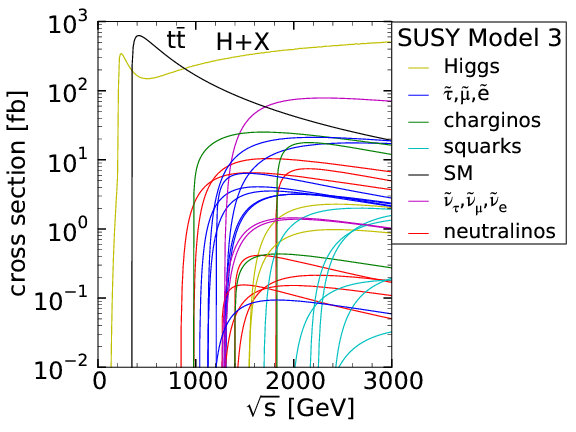
\includegraphics[width=0.75\textwidth,height=10cm,keepaspectratio]{fig/clicSS}
  \caption[Cross Sections For Super Symmetric Processes]{Cross sections for production of various super symmetric particles at an ${e^+e^-}$ collider as a function of centre of mass energy.}
  \label{Fig:SuperSym}
\end{figure}

\subsection{Acceleration Technology}
Unlike \ac{ILC}, the acceleration technology will not be superconducting and will use two beams of electrons-- referred to as the main beam and the drive beam-- rather than just one main accelerated beam. The drive beam is accelerated using standard accelerating technology (Klystrons) as in \ac{ILC} to accelerate bunches of electrons to 2.75GeV. These bunches then enter a series of delay/control rings which are designed such that the electrons within them get combined with the new electrons being added from the drive beam accelerator to build up a large number of low energy electrons which combined have a large energy. The energy from this beam is then used to drive the main beam. This is done by rapidly decelerating the drive beam electrons down to 10\% of their initial energy and using the lost energy (emitted as photons) to accelerate the smaller number of electrons in the main beam resulting in a sudden rapid acceleration. The main beam is then used for the collisions. This approach allows for very high accelerating gradients but has the disadvantage that in approximately 1\% of events the sudden input of energy from the drive beam can cause electrical breakdowns in the main accelerator, which disrupt the alignment and structure of the main beam.

\chapter{Detectors}
The \ac{ILC} has been designed with the intention that it will have two unique detectors so that results can be validated by cross-checking between the two detectors. However, because \ac{ILC} is a linear collider it is only feasible to have one interaction point and as a result the beam time will have to be shared between the detectors. This will be done using a 'push-pull' design in which both detectors are placed on a single platform at the interaction point which can be moved back and forth to position the desired detector in the path of the beams. While having two detectors is certainly desirable as it allows us to get two independent sets of results for the collider and allows us to still take results when one of the detectors requires maintenance, it also has disadvantages as it means an increase in the dead time of the machine (as swapping the detectors is a slow process taking several days which will be done multiple times a year) and an increase in the cost of the experiment. As a result the possibility of using only one detector is still being considered as a potential option. The possibility of splitting the main beam and having two IPs is also being proposed so that both detectors could be used simultaneously however this would be expensive as extra tunnels would have to be built to accomodate this and there would also be a reduction in the beam quality as splitting the beam would produce synchotron radiation.
\section{ILD}
\begin{figure}
  \centering
  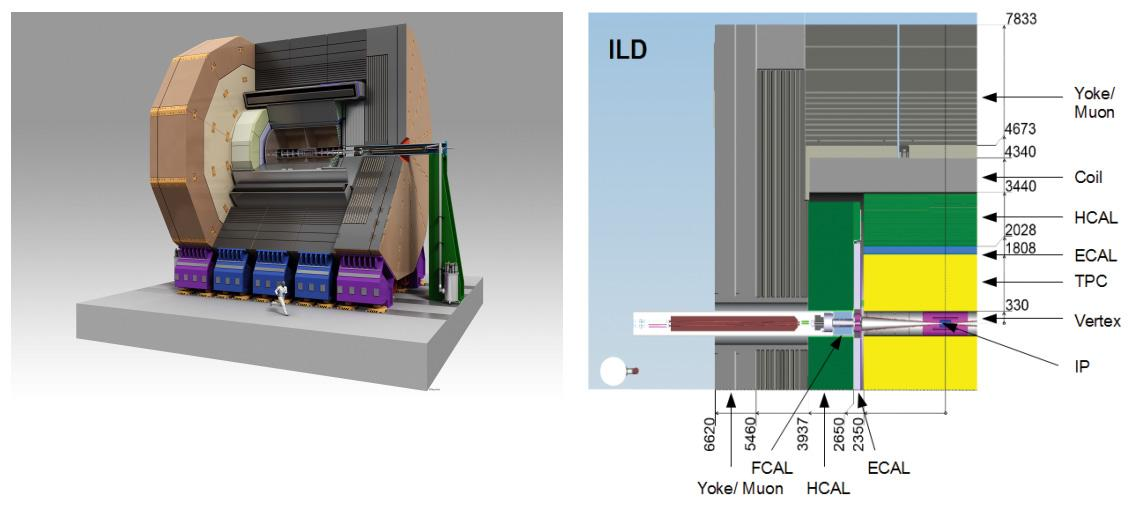
\includegraphics[width=0.95\textwidth,keepaspectratio]{fig/ILD}
  \caption[ILD Detector]{The International Large Detector Concept (left). Schematic of the ILD showing the key components in a one-quarter view of a vertical section of the detector (right). \cite{ILCTDR}}
  \label{Fig:ILD}
\end{figure}
The ILD (shown in \reffig{Fig:ILD}) is a general purpose detector which is cylindrical in design with radius 8m and length 14m. The different sub-detectors are arranged in a concentric manner in the main barrel of the detector, and are positioned with the vertexing technology closest to the beamline, followed by trackers, then electromagnetic and hadronic calorimeters, then the magnetic field coils and finally muon tail catchers. The detector has two endcaps at each end of the barrel creating a hermetic seal. Because many of the physics processes at \ac{ILC} involve Z and W bosons, one of the main performance requirements is the ability to distinguish between the two particles which means achieving a 3-4\% uncertainty in the energy of 100GeV jets and a ${\delta p}$/${p^2}$ (where $p$ is the momentum of a charged particle) of ${5\times10^{-5} (GeV/c)^{-1}}$. All specifications for the detector can be found in the \ac{ILD} Letter of Intent \cite{ILD}. Here we will give a brief overview of the key components and their functions.

\subsection{Vertexing}
The vertexing technology is used to gain information about heavier particles such as b-quarks which have very short lifetimes ($\sim$10$^{-12}$s) and so decay close to the beamline before they can reach the trackers or calorimeters. As such, the vertexers are placed extremely close to the beamline and work by looking for displaced vertices from the initial \ac{IP} which correspond to the point at which the heavy flavour paricles decayed. Due to their proximity to the beam line it is always necessary for the vertex detectors to be very radiation hard as they are exposed to stray high energy particles from the beam. The vertexers also act as trackers for short lived particles that fail to reach the main trackers and so are required to be highly granular to separate particles that have had very little time to spread out since the \ac{IP}. The design for the vertex detectors is yet to be finalised as there are numerous competing technologies under consideration but it is expected to consist of either 3 or 5 cylinders of sensors starting at a radius of $r=15$mm from the beamline.

\subsection{Tracking}
Tracking at the \ac{ILD} uses a \ac{TPC}. This is a large gas filled cylinder with an electric field across it and readout electronics at each end of the cylinder. As particles pass through the gas, they ionize it producing charged particles. The electric field then causes these particles to drift to each end of the detector where they are collected by the electronics. By measuring the position and time at which the charged particles arrive, the track of the original ionizing particle can be reconstructed. A magnetic field is also generated across the chamber to deflect the charged particles so that the momentum and charge of the particle can be estimated. The magnetic field used in the ILD is a 3.5T coil placed outside the calorimeters to minimize the material budget in front of the calorimeters. To gain extra precision on the entry and exit points of the \ac{TPC}, the chamber has two silicon detector layers referred to as the \ac{SIT} and \ac{SET} positioned  immediately before (r=165mm) and after (r=1833mm) the \ac{TPC} which give two high spatial resolution points for the entrance and exit points of particles. These high spatial resolution points are particularly useful for reconstructing individual particles within jets using the Pandora \ac{PFA} (see \refsec{Pandora}.)

\subsection{Calorimetry}

The function of calorimeters is to measure the energy of particles. The ILD uses sampling calorimeters which work by having alternating layers of a dense absorber material that destroy the incoming particle causing it to shower into lower energy particles and active sensor materials which collect the low energy particles and convert them into an electrical signal. The calorimeters are split into electromagnetic and hadronic sections in which the absorbing material is chosen to interact mainly with particles through electromagnetic or strong interactions respectively. In practice this means the \ac{ECAL} mainly detects electrons and photons while the \ac{HCAL} mainly detects hadrons such as pions. Neutral hadrons are recorded exclusively in the \ac{HCAL}.

The ILD ECAL is a highly granular calorimeter poitioned at r=1847mm and consists of 30 active layers separated by layers of tungsten which acts as the absorbing material. The structure of the \ac{ECAL} is shown in \reffig{Fig:ECAL}. The choice of active material is yet to be made though the two leading techologies are silicon scintillators or pixels. The scintillator form of the technology uses 10x45mm strips which would be rotated by 90${^o}$ in each successive layer to produce an effective cell size of 10x10mm with photomultipliers attached to each strip for readout. This form of the technology is considerably cheaper but has a lower performance and relies on algorithms accurately correlating hits in successive layers to produce the effective 10x10mm cell size. The pixel form of the technology simply uses 5mm or 10mm square silicon pixels directly connected to the readout electonics. This is more expensive but produces more consistent results.

\begin{figure}[h]
  \centering
  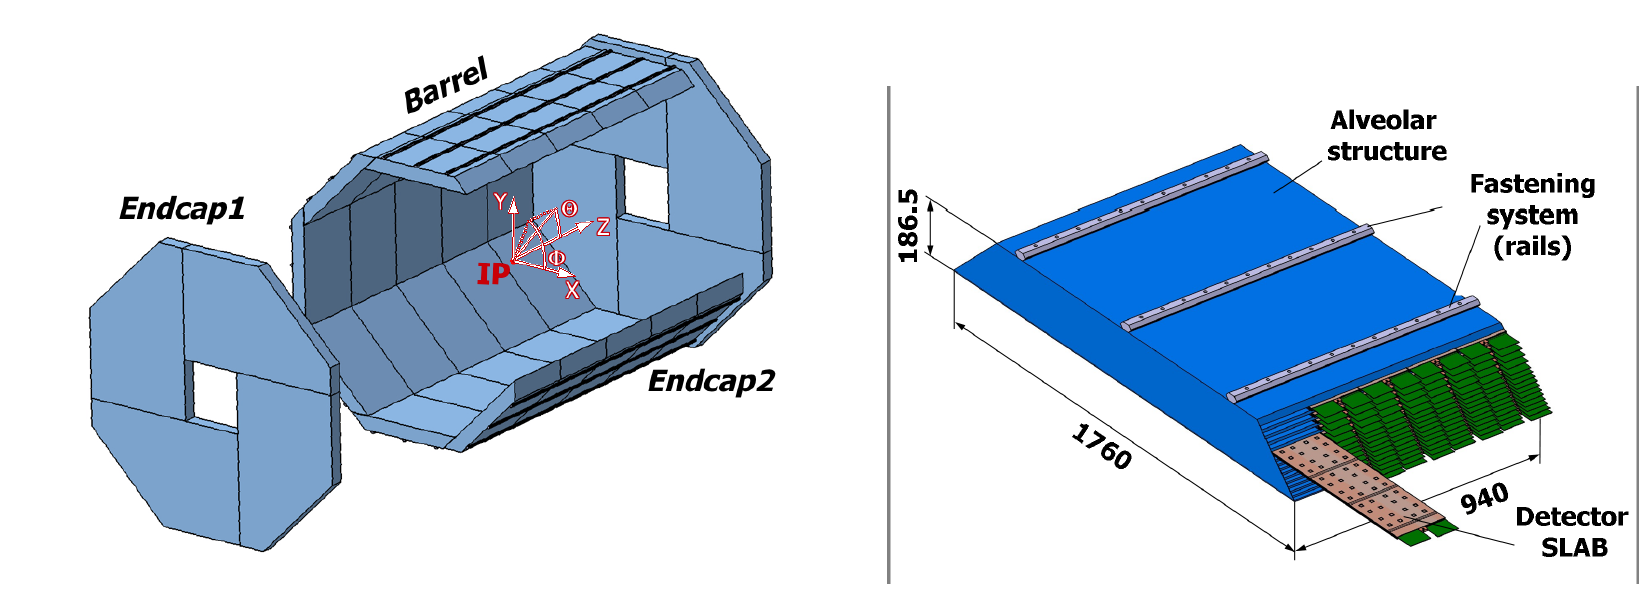
\includegraphics[width=0.95\textwidth,keepaspectratio]{fig/ecalstructure} %aw replace image with higher quality version
  \caption[ECAL Structure]{The Overall ILD Structure (left) and one individual module (right).The ECAL is made up 40 modules, each containing 30 detector slabs. The modules are combined into groups of 5 referred to as a stave whih extend along the full length of the barrel. There are then 8 of these stave arranged in a circle to create the circumference of the barrel \cite{ILD}.}
  \label{Fig:ECAL}
\end{figure}

Later on (see \refsec{Sect:DECAL}) we will discuss our work on developing an alternative form of the silicon pixel technology with a cell size of 50x50${\mu}$m which acts as a digital machine and purely counts the number of particles absorbed in the active medium from the showering in the absorber and deduces the energy of the original particle from this.  This form of the technology has already begun to be studied \cite{2011JInst...6.5009B}. It is expected to be cheaper than the standard silicon pixel tehnology and has already been shown to produce no significant decrease in performance.

The \ac{HCAL} is immediately outside the ECAL at r=2058mm and has a similar overall modular structure. The HCAL uses stainless steel as an absorbing medium combined with scintillators and Silicon PhotoMultipliers. Again both digital and analogue variations are available with the analogue using 3x3cm cells and the digital 1x1cm. The relative performance of each technology is still being evaluated to see if there is any degredation in the performance when using the digital variation.

\subsection{Muon Detection}
Muon detection is perhaps the easiest process to perform at the ILC. Because the signal events at the ILC are clean with few high energy particles, few particles other than muons are capable of penetrating through the inner detector layers and the coil generating the magnetic field. As a result the muon detetors are produced by instrumenting the return yolk (r=4424) that already surrounds the detector to contain the magnetic field. The number of muons produced in an event is also relatively small which means that the cell size for the muon detectors can be moderately large without the risk of multiple occupancy. The instrumentation is done by placing 10 layers of resistive plate chambers into the return yolk with strip sizes of the order 3-4cm. This system is sufficient for accurately detecting muons and contributing to the measurement of their momentum.

\section{SiD}

\begin{figure}
  \centering
  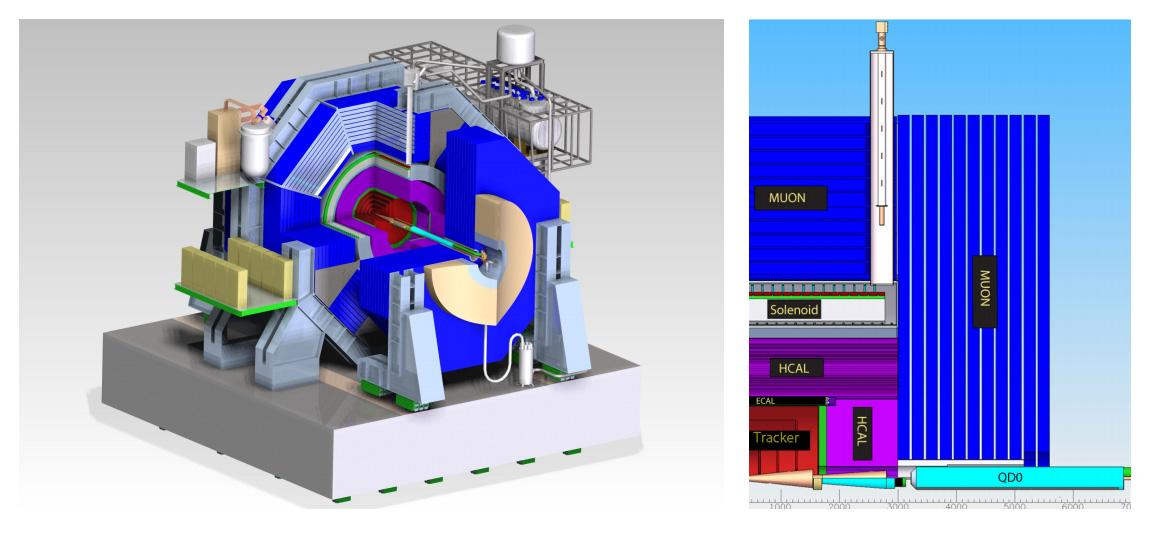
\includegraphics[width=0.95\textwidth,keepaspectratio]{fig/SiD}
  \caption[SiD Detector]{ The Silicon Detector Concept (left). Schematic of the SiD showing the key components in a one-quarter view of a vertical section of the detector (right). \cite{ILCTDR}}
  \label{Fig:SiD}
\end{figure}

The \ac{SiD} (\reffig{Fig:SiD}) is overall quite similar to ILD with the two main differences being that SiD uses a stronger 5T magnet and a different form of tracking. Tracking at the SiD uses silicon strips rather than a TPC. This results in a better performance but is considerably more expensive. As this is the only signifcant difference from ILD we will not go into any further detail about the subdetector technologies used for SiD.

\chapter{Linear Collider Analysis Framework}

Before discussing the work we have done this year, it is useful to have a brief overview of the software used for linear collider analysis. Both \ac{ILC} and \ac{CLIC} use the same core set of packages referred to as ILCSoft. This shared framework makes it easy for work done for one experiment to be ported for use in the other which is beneficial for both experiments as it reduces the amount of work needed for each and helps prevent duplication of efforts. Here we will give an overview of the most commonly used packages in ILCSoft.

\section{Mokka}
Mokka is a Geant4 based simulation package available in ILCSoft. Mokka allows users to take ``.stdhep'' files created from an event generator such as PYTHIA or WHIZARD, simulates how a detector will respond in the presence of the events and outputs info such as calorimeter and tracker hits into a ``.slcio'' (the standard linear collider file format.) Standard detector geometries are stored in a database online from which Mokka extracts them at runtime. The geometry is modular in design with components such as the ECAL and TPC described separately. Users are able to customize the detector for simulation studies by replacing the standard detector components with an alternative version. The modules can even be customized manually in the Mokka steering file e.g. the number of layers in the ECAL or the thickness of the sensitive layer in the HCAL can be changed. Mokka will then automatically try to resize the customized component to make it fit in the appropriate space within the larger detector design. As well as accepting ``.stdhep'' files Mokka also has an inbuilt ``particle gun'' which can be used to fire particles with any energy at any position within the detector. This tool is particularly useful for studying a particular component of the detector without worrying about the effect of any of the components between it and the \ac{IP}.

\section{Pandora Particle Flow Algorithm}
\label{Pandora}
Pandora is an advanced Particle Flow Algorithm used at linear colliders which allows an increased level of precision from detector measurements by combining information from all the different detector components. The main aim of a \ac{PFA} is to associate calorimeter hits with individual tracker hits using topology then use the tracker information to calculate the particles' energy, as there is less uncertainty on this than on the measurement by the calorimeter. If there is ambiguity when associating tracks with hits (e.g. in jets) then the \ac{PFA} will instead use the calorimeter to determine the particles energy. Because we ideally want to use the track measurements for every particle the performance of the \ac{PFA} is boosted by having a high spatial resolution measurement at the end of the tracker (e.g. the \ac{SET} in \ac{ILD}) and having a high granularity calorimeter at the start of the \ac{ECAL} as this reduces the ambiguity when associating tracks with calroimeter hits. The optimization for \ac{PFA} has been one the main influencing factors for the design of the detectors at ILC and CLIC. In ILCSoft Pandora is implemented in Marlin (see below) and is used to convert the hits output by Mokka into reconstructed particles referred to as \ac{PFOs}.

\section{Marlin}
Marlin is the main analysis tool in ILCSoft. It is a modular framework which applies a series of processors to an event where each processor can be built separately to perform a seperate task. For example one processor might perform jet finding while another might carry out lepton finding. Marlin is controlled with xml steering files containing a list of the processors to be used, the lcio files on which Marlin will act, the detector geometry used by Mokka and the parameters which the processors need e.g.\ energy cuts or jet radius. The main benefit of the Marlin system is the ability to ``plug and play'' by which we mean processors can be added/removed and their parameters can be changed in the Marlin steering file to change the analysis at any time without having to recompile any code. Processors from one analyis can also be used in another analysis simply by including them in the steering file with the idea being that eventually there will be a large database of processors which users can pick and choose from without having to construct their own. The ILCSoft installation already comes with standard processors that link in to FastJet (jet finding), LCFIPLUS (flavour tagging), Root and Pandora.

A typical analyis from start to finish might proceed as follows:
\begin{itemize}
\item Generate event with Whizard, output is stdhep file
\item Simulate event in detector with Mokka, output is lcio file with raw detector hits
\item Apply Pandora PFA using Marlin, output is lcio file containing reconstructed particles
\item Perform Analysis using Marlin, output is Root ntuple containing parameters like missing energy, number of jets etc 
\end{itemize}

\chapter{Studies Performed at Birmingham}

\section{Longitudinal Shower Profiles}
One of the most straightforward ways to characterize a calorimeter is in terms of how much of a particles' energy will be collected in it and how deep the calorimeter must be in order to contain the entirety of the particles' energy. Here we have performed this type of characterization for the standard ECAL for the ILD described in the geometry model ILD\_o1\_v05 which uses 30 layers of detectors. This was done using the particle gun in Mokka to fire particles directly into the calorimeter. The particle gun produced particles 5cm in front of the ECAL at a position far from the boundary between modules to ensure that particles were all entering the same module at right angles. Initial tests were done by firing 20 GeV muons at the detector to check our system for analysis was correct. The results from this showed a uniform distribution of energy between all the ECAL layers corresponding to approximately one hit per layer per muon as expected. Following this we then fired a sample of 20,000 5GeV electrons then 20,000 5GeV photons at the ECAL to measure its response. Photons and electrons were chosen as they are the dominant types of particles the ECAL is used to detect. The results for this are summarised in \reffig{Fig:showers} and \reftab{Tab:showerstab}.

\begin{figure}[h]
  \centering
  \subfloat[]{ 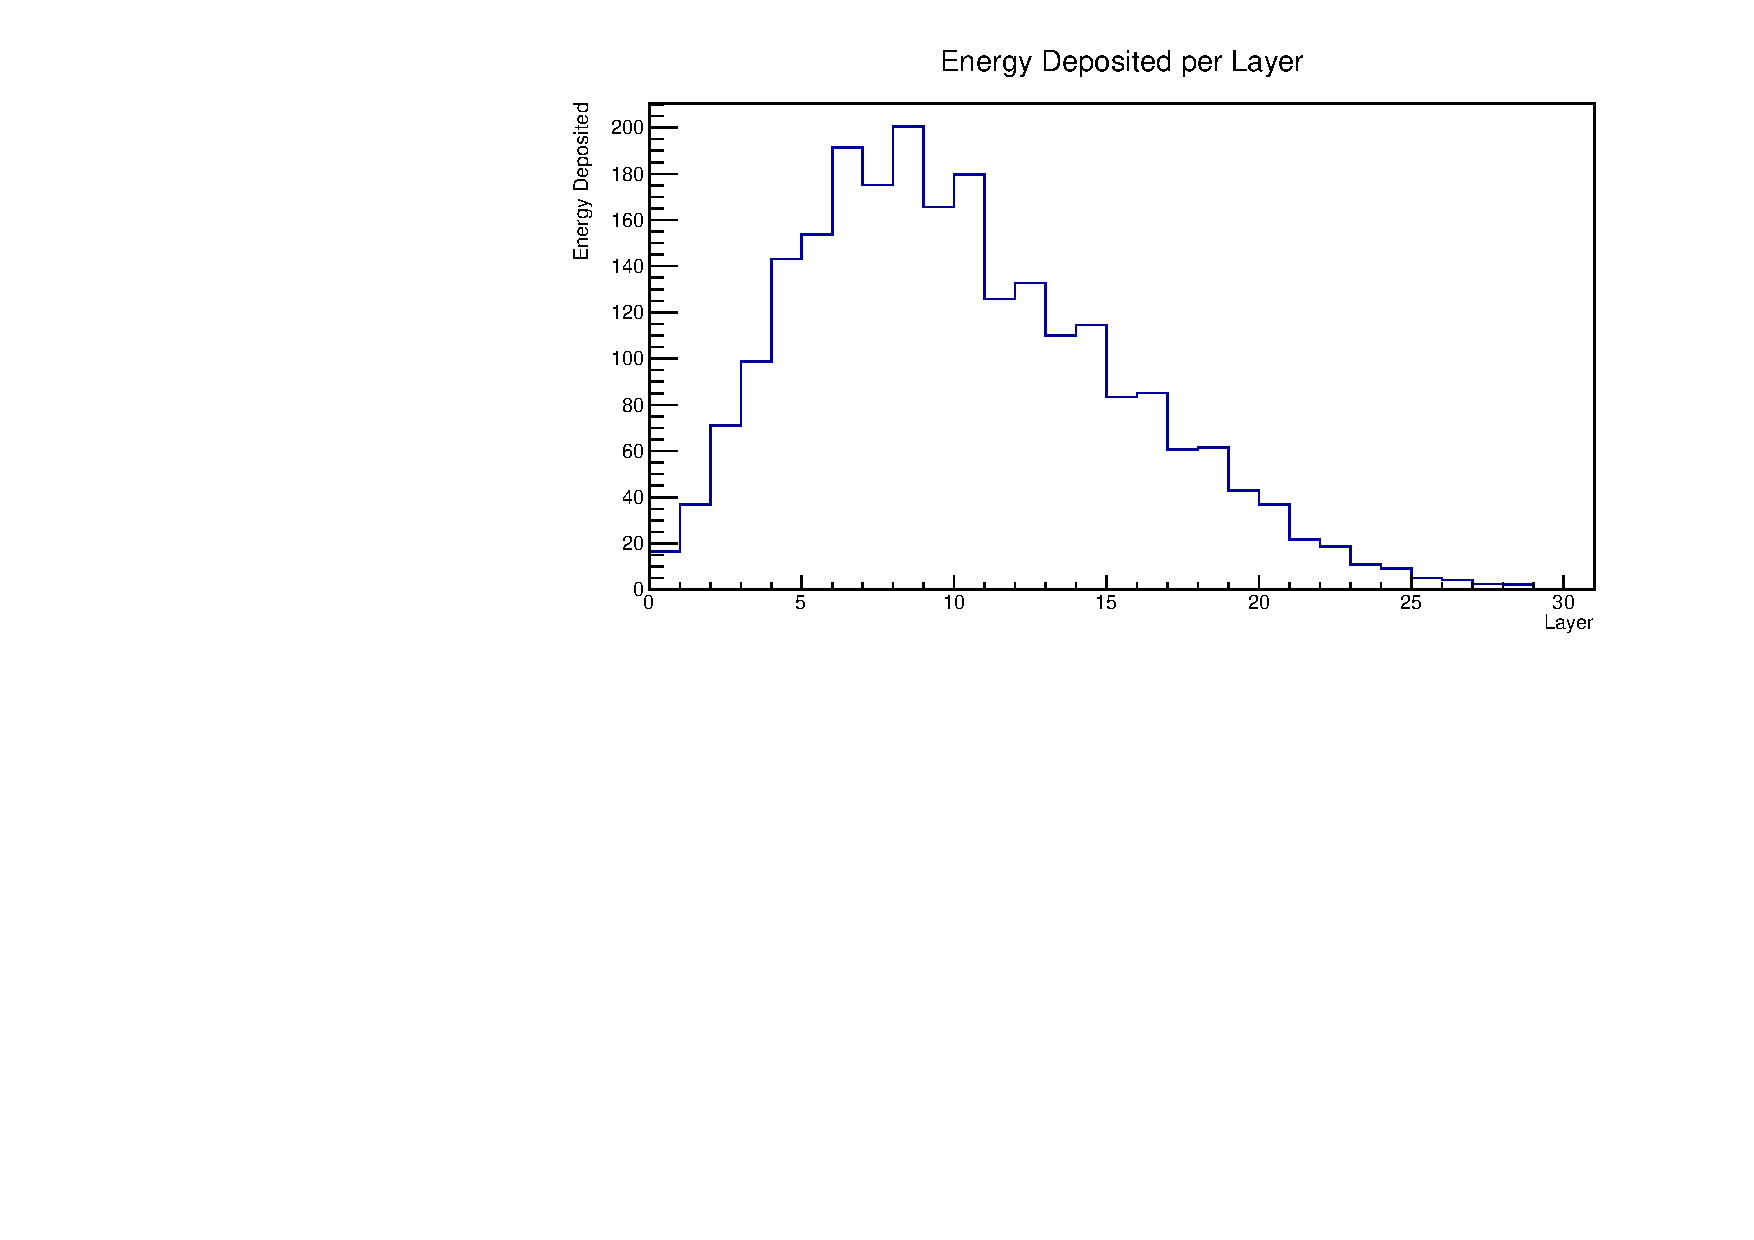
\includegraphics[width=0.52\textwidth,height=7cm,keepaspectratio]{fig/longitudinalelectrons}}
  \subfloat[]{ 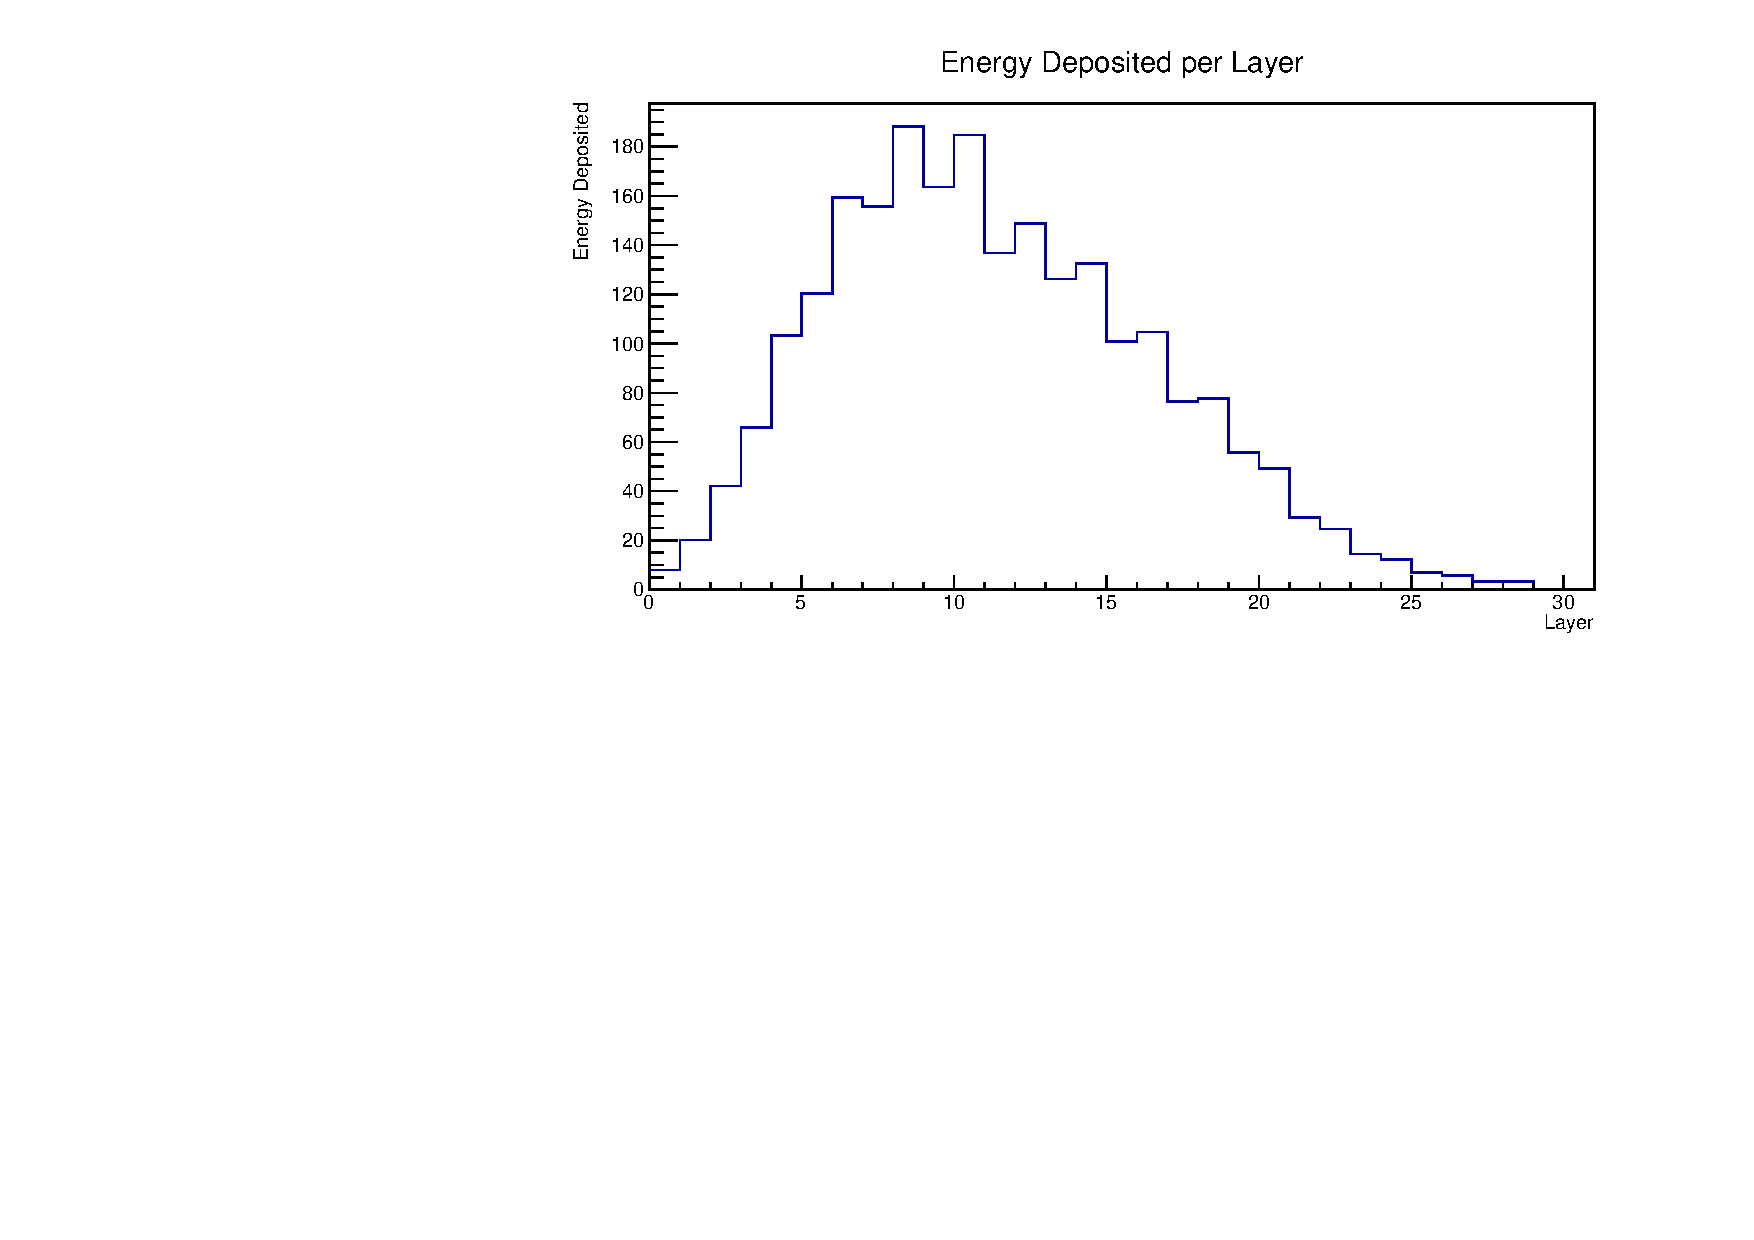
\includegraphics[width=0.52\textwidth,height=7cm,keepaspectratio]{fig/longitudinalphotons}}
  \caption[Longitudinal Shower Profiles For 5GeV Electrons and Photons]{Longitudinal Shower Profiles for 5GeV electrons(left) and photons(right).}
  \label{Fig:showers}
\end{figure}


\begin{figure}[h]
  \centering
  \label{Tab:showerstab}
  \begin{tabular}{l p{0.3\textwidth} p{0.35\textwidth}}
    \toprule
    ~     & Layer Containing 90\% of Deposited Energy  &   Fraction of Deposited Energy Contained by ECAL        \\
    \midrule
    5GeV Photon Events                & 19      & 99.47\%    \\ 
    \midrule
    5GeV Electron Events              & 18      & 99.61\% \\
    \midrule
    \bottomrule
  \end{tabular}
  \caption[ECAL Performance]{The number of layers necessary to contain 90\% of the total deposited energy and what fraction of the total deposited energy the ECAL successfully contains. Note that layer counting starts at zero.}
\end{figure}

The performance of the ECAL is clearly satisfactory with virtually no energy leakage into the HCAL and over 90\% of the energy being absorbed within the first 20 layers of the detector. These diagrams also highlight that there is a discrepancy between even and odd numbered layers. This is because the ECAL detectors are structured in such a way that the active layers are in pairs where the material budget between two layers in a pair is different than the material budget between one pair and the next pair. This means that particles have to travel through more material to reach one set of layers than the next and so there is a difference in the energy collected. In practice however the measured energy for a particle is the sum of all the layers and so it is not so important where the layers are within the detector.

In future we may look at repeating this experiment at different energies to see how the efficiency of the calorimeter depends on the energy of the incident particles.

\section{Digital ECAL}
\label{Sect:DECAL}

\subsection{Analogue Calorimetry vs Digital Calorimetry}

In traditional analogue calorimetry, measurements are performed by summing the energy deposited in each of the active layers of the calorimeter to find the rate of energy loss of the incident particle, scaling this by an efficiency factor that has been measured during calibration of the calorimeter, then using the theory of shower development and the known properties of the materials in the detector to determine the incident particle energy. While this method is normally satisfactory, the resulting energy mesurement will have a relatively large uncertainty due to the fact the energy deposited by a particle in the active material is influenced by many factors such as the incident angle of the particle and the fact that showering is a statistical process. Digital calorimetry acts in a similar manner but instead of measuring the energy deposited in the calorimeter, you count the number of hits in the detector (number of particles in the shower) then use the fact this is proportional to the energy of the incident particle. While this method still has some uncertainty from the conversion factor of hits to number to energy of incident particle it has been shown that this uncertainty is smaller than in analogue calorimetry \cite{Price:2012vta}. While digital calorimetry offers the potential for more precise energy measurements, it will only work if the detector can distinguish individual particles within a shower. If the pixel size for the calorimeter is too large then it is possible that multiple particles will hit the same pixel and because the detector uses binary readout, it will only register the presence of a single particle and so the number of particles will be underestimated and hence the energy calculated will be less than the true energy of the particle. The peak shower density in the ILC ECAL is expected to be 100particles/${mm^2}$ and so a pixel size of at most 50x50${\mu}$m will be necessary to avoid multiple occupancy of pixels.

\subsection{Cherwell Sensors}

So far our hardware studies have been focused on characterizing novel high granularity sensors referred to as Cherwell sensors (\reffig{Fig:cherwell}) which are based on standard CMOS \ac{MAPS} technology. Each sensor is 5x5mm and contains 4608 pixels. The pixels are then divided into four sub categories- two sets of DECAL pixels (25x25${\mu}$m and 50x50${\mu}$m) which have an external \ac{ADC}, a set of reference pixels and strixels which have an integrated \ac{ADC}. The ones we are most interested in are the two sets of DECAL pixels. The 50${\mu}$m pixels are the standard size for use in the DECAL while the 25${\mu}$m pixels are designed for the possibility for standalone use in the vertexers/trackers then ganging together into groups of four to create a virtual 50${\mu}$m pixel for the DECAL. The possibility for ganging the smaller pixels together is yet to be fully tested but would be beneficial as it would simplify the detector design by allowing one technology to be used for multiple components. CMOS based sensors are also considerably cheaper than other sensors due to the widespread use of CMOS devices in everyday technology. 

\begin{figure}
  \centering
  \subfloat[]{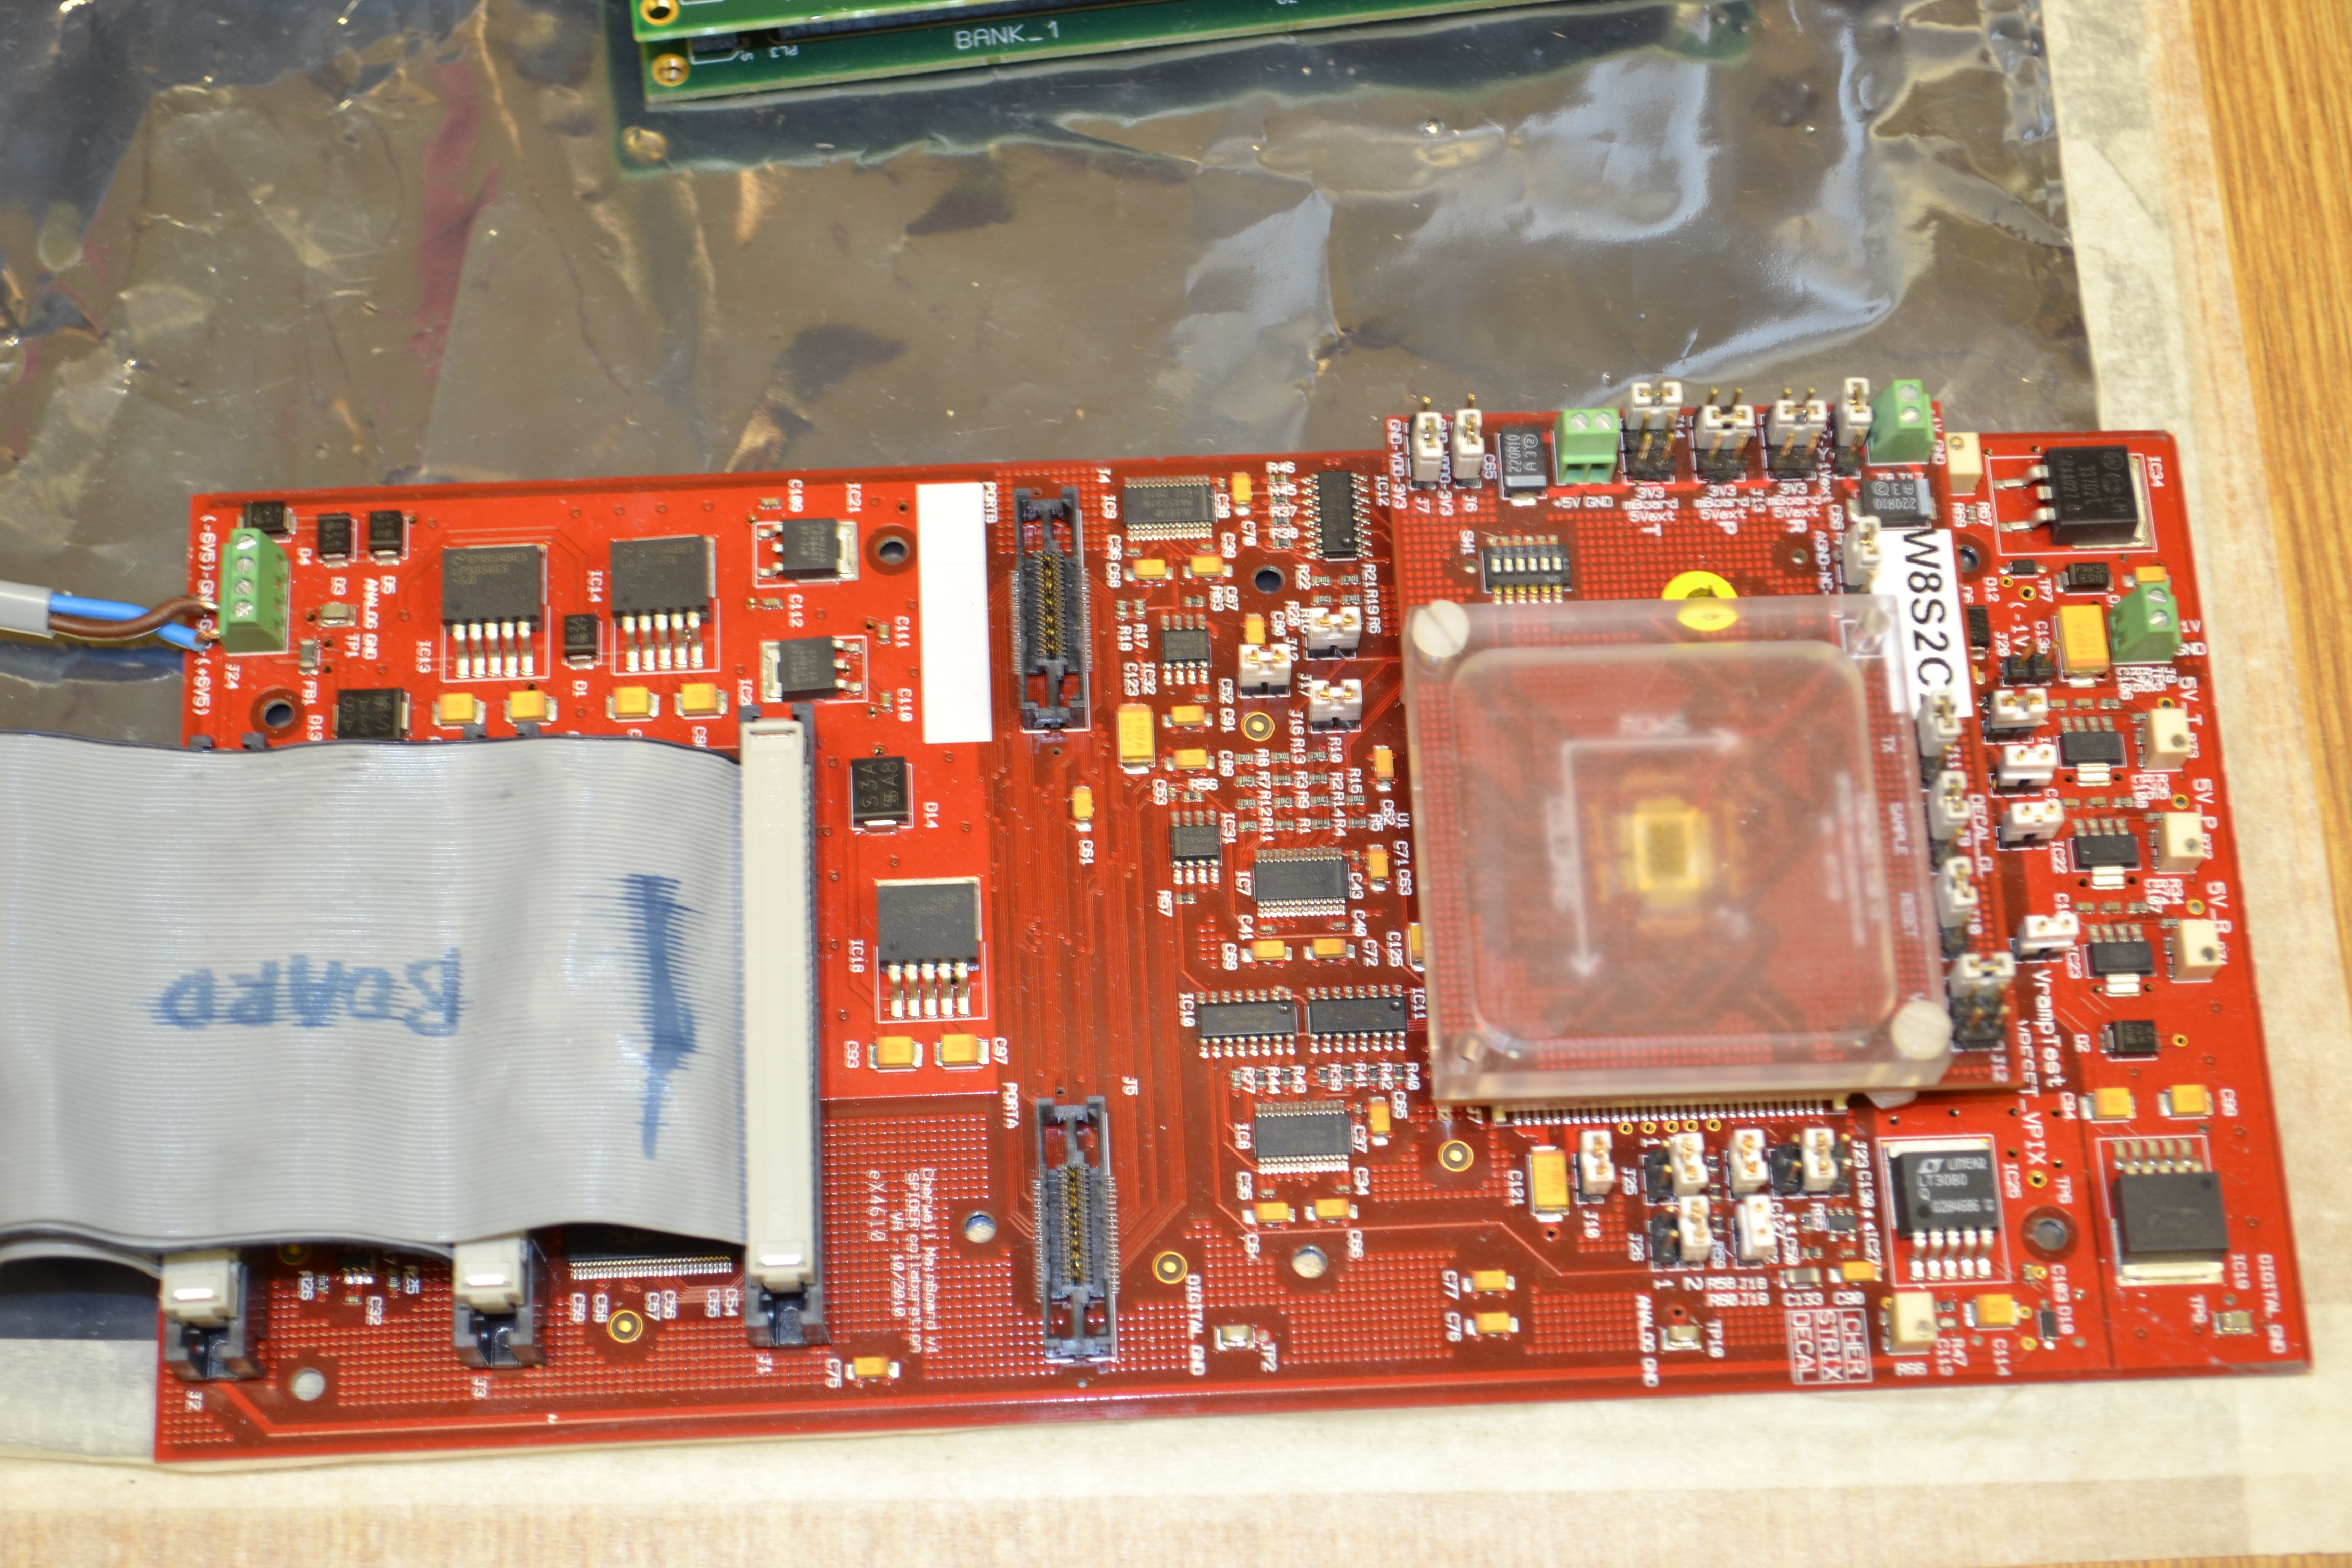
\includegraphics[width=0.4\textwidth,height=7cm,keepaspectratio]{fig/cherwell}}
  \qquad
  \subfloat[]{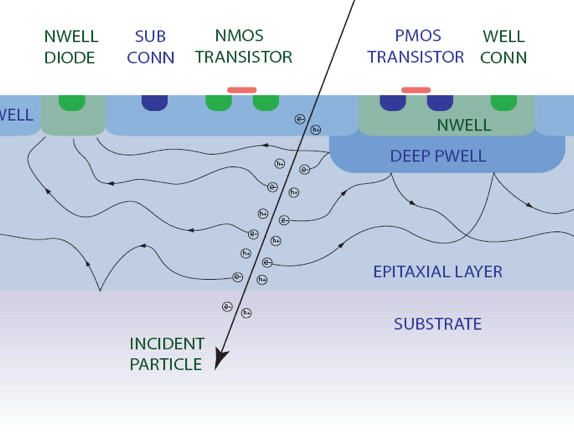
\includegraphics[width=0.4\textwidth,height=7cm,keepaspectratio]{fig/deeppwell}}
  \caption[The Cherwell Sensor]{The Cherwell sensor. The Cherwell sensor uses a high resistivity 12${\mu}$m epitaxial layer (1-10k${\Omega}$cm) to speed up charge collection and a deep p-well surrounding the n-well of the PMOS component to prevent charge being diverted from the nwell diode \cite{MylroieSmith}.}
  \label{Fig:cherwell}
\end{figure}

Our current setup for the Cherwell is shown in \reffig{Fig:basement}. This setup is copied from that used at \ac{RAL} where testing of the strixel components of the Cherwell has been undertaken. As a result, some of the features of the setup are not being used by us, namely the discriminator is designed for using the sensor with scintillator/photomultiplier triggers which we currently do not have, and the external clock is designed for use as a master clock when using multiple sensors at once while we are only using one board. Our sensor currently uses a rolling shutter with the external trigger running at 5Hz to trigger the DAQ readout. The trigger system will be upgraded in the autumn to allow an internal trigger instead of the external trigger as we currently only have one external trigger board which, if broken, cannot be replaced. The DAQ system for the Cherwell reads out the raw ADC hits from the Cherwell board in gray code without any thresholds or corrections applied to the hits. The thresholds and data correction are therefore done afterwards during analysis fo the data.

Due to damaged components and outdated firmware, the studies we have carried out are still at the early stage of getting raw ADC hit maps with no zero-suppression or common mode corrections performed on them. Our future work will be aimed at testing features of the Cherwell sensor that wil be necessary for usage in the \ac{ILC}. In particlular we will be studying the effect of ganging the 25${\mu}$m pixels together discussed above to see if there is a degredation in the performance when doing this as well as looking at the effect of power pulsing on the detector, as mentioned in \refsec{ILC:BEAM}. Due to the collision rate of the \ac{ILC}, the duty cycle for the detector will be just 1\% meaning that the detectors can be powered down for up to 99\% of the running time. This reduces the need for elaborate cooling systems as the heat generated by the electronics in the machine will have enough time to cool down passively. However if the electronics are only on for a short time there is a chance that there will be a degredation in performance as the sensors will need some finite time to settle. Hence it is necessary for us to examine the performance of the sensors for various duty cycles to determine the minimum time period required for the sensor to reach equilibrium. 

\begin{figure}
  \centering
  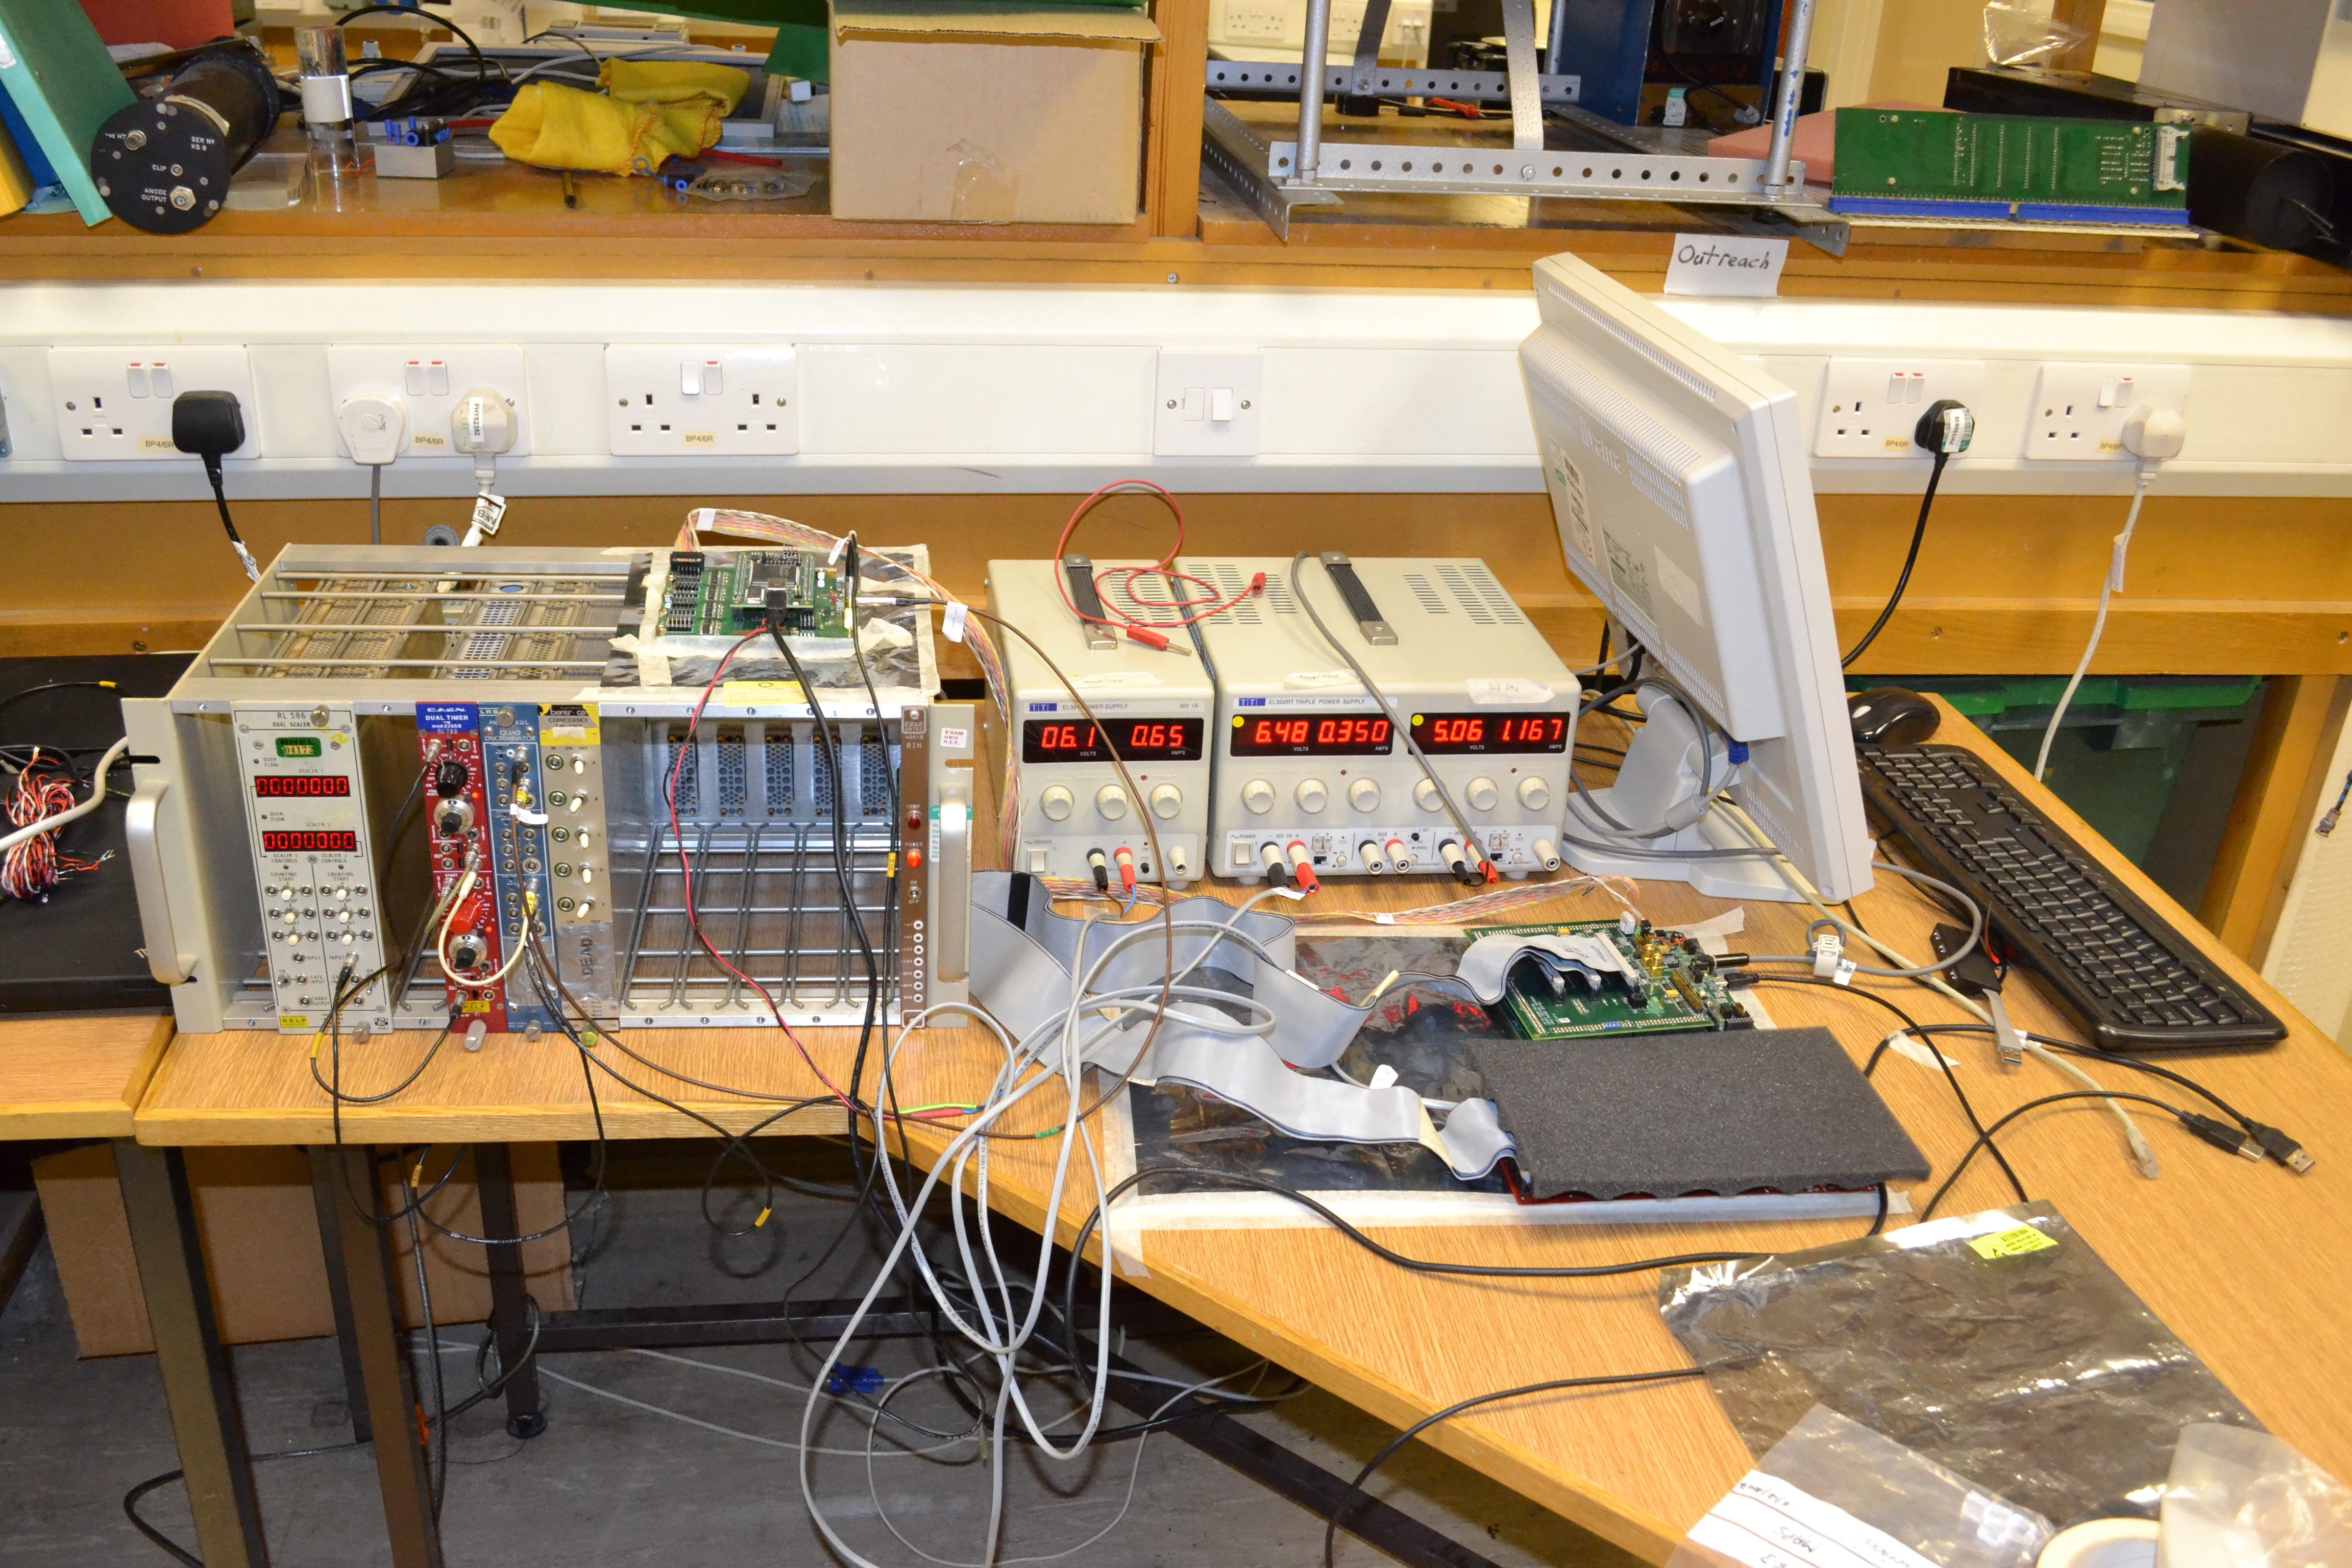
\includegraphics[width=0.48\textwidth,height=7cm,keepaspectratio]{fig/basement}
  \caption[Birmingham Cherwell Sensor Setup]{The Birmingham Cherwell Sensor Setup. The Cherwell sensor is in the lower right under a layer of black foam for protection. The DAQ board (green) is positioned behind the sensor. To the left is a NIM crate containing a discriminator and clock signal generator  with the external trigger attached on top. Three seperate power supplies connected to a common ground are used to power the sensor, trigger and daq boards separately.}
  \label{Fig:basement}
\end{figure}

\section{Measurement of the H${\rightarrow}$WW* Branching Ratio}

The bulk of work done in our first year has been an analysis with the aim of measuring the H${\rightarrow}$WW* branching ratio. We have decided to look at the mode in which a Higgs is produced via WW-fusion then decays to a pair of Ws which decay semileptonically (see \reffig{Fig:feynmann}). The samples used for this have been for 1.5${ab^{-1}}$ of 1.4TeV collisions at \ac{CLIC} using the \ac{ILD} detector. The samples we have used from the \ac{CLIC} database are PROD\_ID 2022 (${e^+e^-\rightarrow H\nu\nu}$ inclusive, cross section 244.1fb) and PROD\_ID 3249 (${e^+e^-\rightarrow qql\nu}$ inclusive, cross section 4309.7fb.) The signal events were then extracted from 2022 and the remaining events combined with 3249 were used as background events. In future we will refer to the different signal and backgrounds as follows:

\begin{itemize}
\item 2022\_Signal - our signal events extracted from PROD\_ID 2022
\item 2022\_Background - the ${h\nu\nu}$ events left over from PROD\_ID 2022 after removing the signal events
\item 3249\_Background - all the ${qql\nu}$ events that make up PROD\_ID 3249
\end{itemize}
The first stage of our analysis was to take our signal events and reconstruct the Higgs particle. This process was done in Marlin with the processors shown in \reffig{Fig:Marlin}. The output of these set of processors is a root ntuple containing various parameters (e.g. Higgs Mass and thrust) measured for each event. The resulting ntuples were then used to train and test neural nets to distinguish signal and background events from each other. Currently we have done the analysis with a small sample to save time, $\sim$30,000 signal events, $\sim$150,000 background events, though we are currently in the process of udgrading our sample size to the full set generated by \ac{CLIC}, 80,000 signal events, 2,000,000 background events, to reduce the statistical uncertainty in our calculations.

\begin{figure}
  \centering
  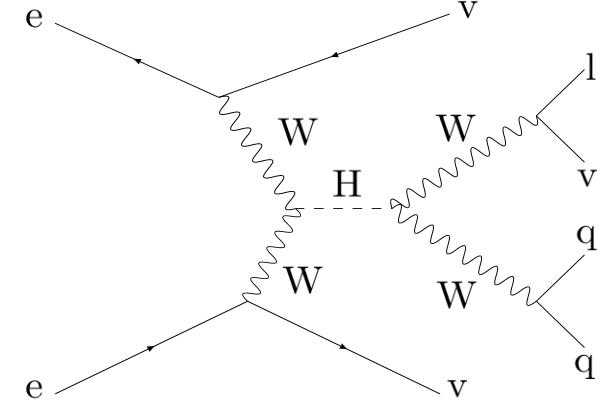
\includegraphics[width=0.48\textwidth,height=7cm,keepaspectratio]{fig/feynmann}
  \caption[Signal Feynmann Diagram]{Higgs produced via WW fusion decaying to a WW pair which decays semileptonically}
  \label{Fig:feynmann}
\end{figure}


\begin{figure}
  \centering
  \label{Fig:Marlin}
  \begin{tabular}{l p{0.6\textwidth}}
    \toprule
    Processor     &     Description          \\
    \midrule
    AIDA       &     Sets up the Root interface to Marlin so results can be output as Root ntuples      \\ 
    \midrule
    FastJet\_kt2jets     &  Uses the kt\_algorithm with R=0.30 to sort all PFOs into 2 jets using the E-scheme for combining particles \\
    \midrule
    PoorIsolatedLeptonFinder &    Uses loose kinematic cuts based on jet and PFO properties to select all possible leptons that might have come from a W-Boson \\
    \midrule
    IsolatedLeptonFinder &      Uses the PID value given by the Pandora PFA to identify all leptons then selects the highest energy one to be the lepton from the leptonic W decay. This lepton is assumed to be the correct lepton for the rest of the reconstruction \\
    \midrule
    FastJet\_kt2Jets &      Sorts the PFOs without the isolated lepton into two jets using the kt\_algorithm with R=0.4 using the E-scheme for combination\\
    \midrule
    FastJet\_kt4Jets &      Sorts the PFOs without the isolated lepton into four jets using the kt\_algorithm with R=0.4 using the E-scheme for combination \\
    \midrule
    ThrustReconstruction &  Calculates the thrust of the entire collection of PFOs   \\
    \midrule
    ThrustReconstructionIsolep &  Calculates the thrust of the PFOs without the isolated lepton    \\
    \midrule
    HiggsWWReconstruction & Combines the two jets into a W-boson then determines it's properties, combines the W-Boson with the isolated lepton then calculates the resulting Higgs Bosons properties.  \\
    \bottomrule
  \end{tabular}
  \caption[Marlin Processors Used For Higgs Reconstruction]{Marlin Processors Used For Higgs Reconstruction}
\end{figure}

\subsection{Optimization of Lepton and Jet Finding}

Lepton finding was optimized by using \ac{MC} information to determine which PFO really came from the leptonic W decay then seeing if the PFOs we tagged as leptons matched this true lepton. Originally we used only the ``poorleptonfinding'' processor which was found to have a purity and efficiency of 74\% and 91\%.\footnote{This means 74\% of tagged leptons corresponded to the true lepton and 91\% of the time the true lepton would be one of the tagged leptons.} This was then improved upon by switching from our own kinematic cuts to using the \ac{PFA} for PID and picking the highest energy lepton to be the one from the W-decay. The new method shows a distinct improvement as it it yields a purity and efficiency of 96\% and 93\%. While this method improves the ability to find the correct lepton for reconstructing the Higgs particle it also has the draw back that the number of particles selected by the processor is virtually always one (in the highly rare case that there are no leptons in an event it will return zero) which means it does not produce a useful variable for distinguishing signal and background events. This is not the case for the ``poorleptonfinder'' which can select multiple leptons and so this is why we still include it in our analysis even though the leptons it selects are not used for any other purpose.

Jets of hadrons are defined by using algorithms that group observed particles together to form a single 4-vector that ideally corresponds to the primary quark. The choice of what value of R to use for our jet finding algorithm was determined again by using \ac{MC} information. This time we used the \ac{MC} to find out the energy of any neutrinos produced in the W decays and add them to our reconstructed Higgs particle. We then varied the R parameter such that the Higgs mass corresponds to the generated Higgs mass used in the simulation. Even though we only expect two jets in our final state, we still include a four jet processor because it will return a value for the resolution parameter in the kt\_algorithm for the transition of the system from 2${\rightarrow}$3 and 3$\rightarrow$4 jets. The value for the resolution parameter at these transition points (referred to as Y23 and Y34) can then be used to distinguish our signal from background processes which produce final states with more than two jets.

\subsection{FlavourTagging}

Before the above processing was done, all events were flavour tagged to help distinguish heavy flavour events which could mimic our signal, e.g.\ events could have a b-quark decaying to a c-quark in association with a W-boson which decays leptonically, giving an isolated lepton similar to our signals. Flavour tagging was implememted using the LCFIPLUS package from ILCSoft which performs vertexing and jet finding based on particle track information then uses a neural net to give two tags (btag and ctag) to each jet indicating the likelihood the jet was produced by a c or b quark. The neural net used requires training before it can be applied. We opted to train the net using events of the type ${e^+e^-\rightarrow Z\nu\nu, Z\rightarrow q\bar{q}}$ with 10000 events for each of q=u/d/s, q=c and q=b. To measure the performance of the neural net we created a purity vs efficiency plot (\reffig{Fig:purity}) for various btag values. The plot shows that a high purity and efficiency can be attained simultaneously indicating that the tagging is working effectively. The neural net was then applied to our signal and background samples and the btag and ctag values for each event were extracted and added to our root ntuple.

\begin{figure}
  \centering
  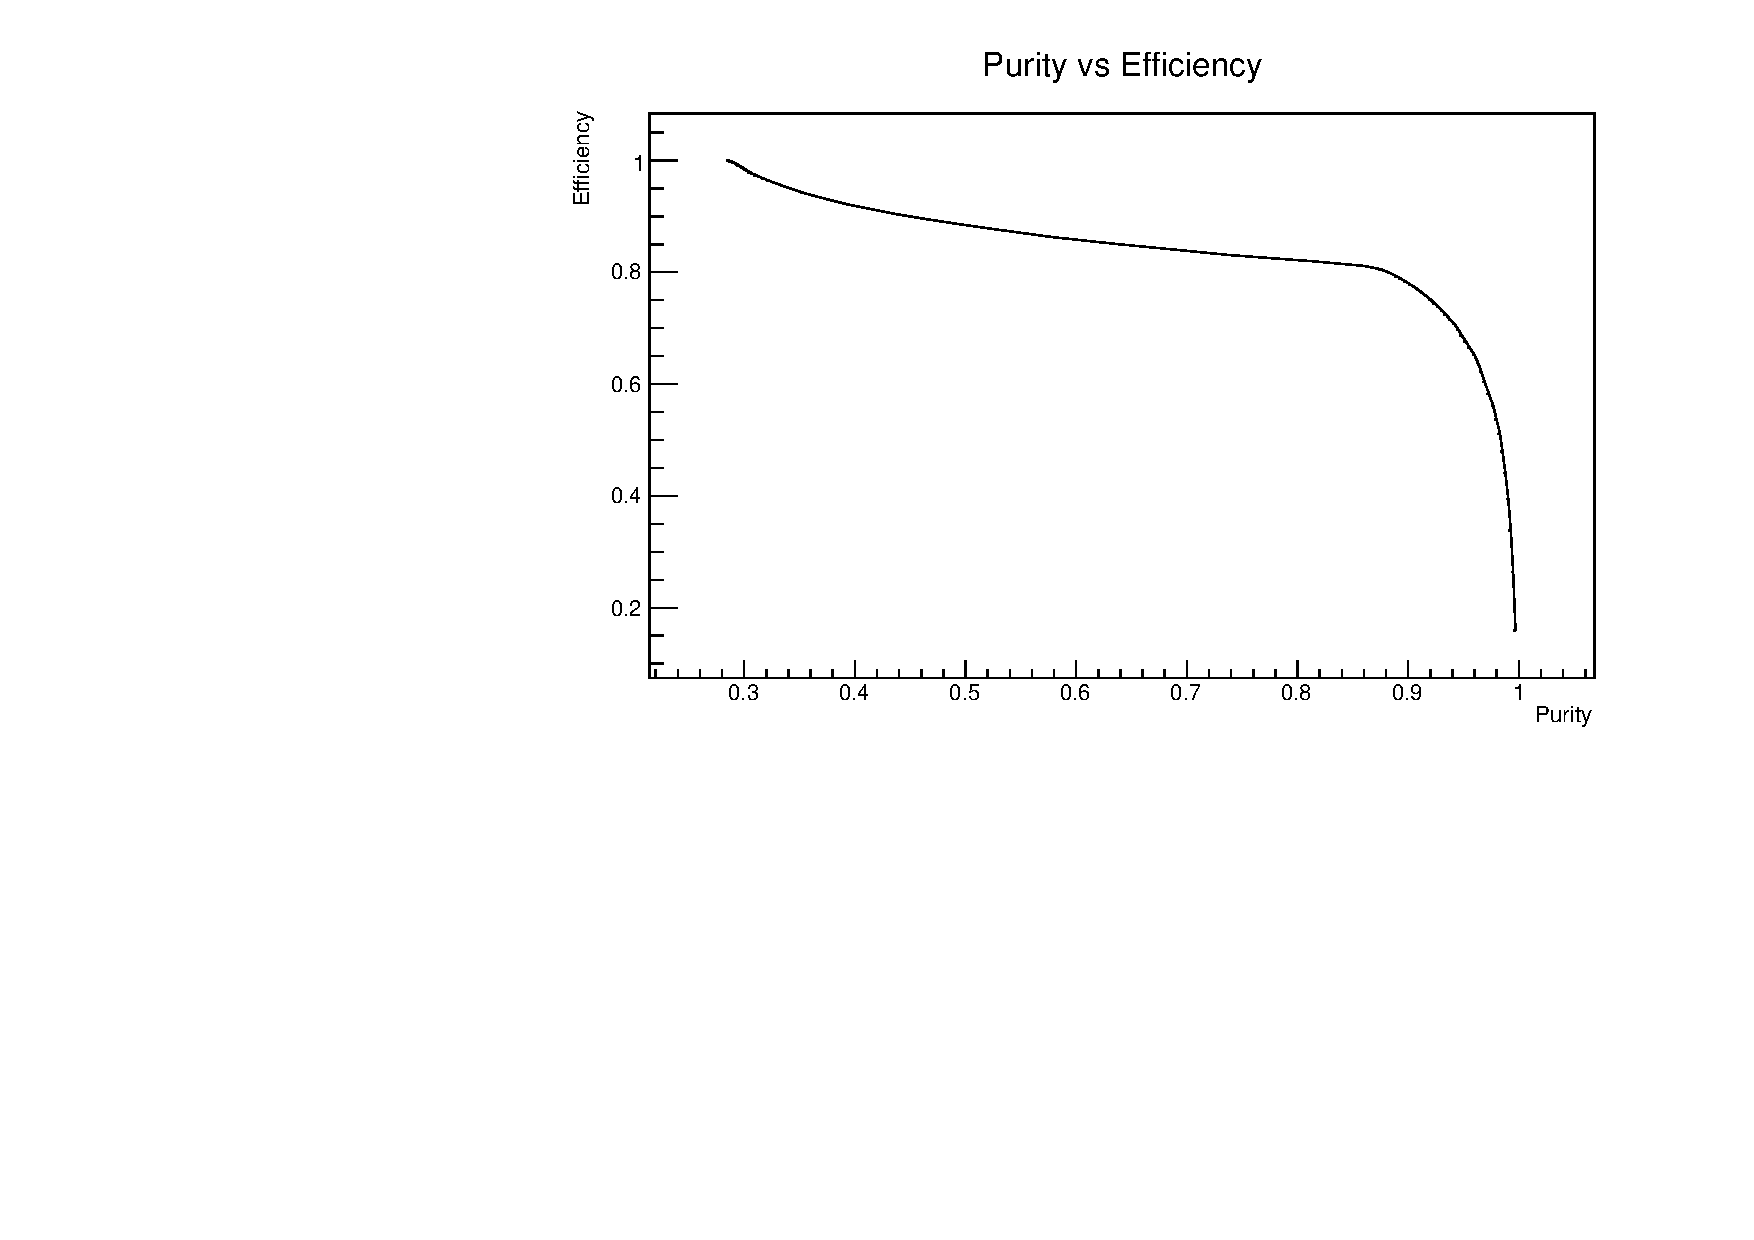
\includegraphics[width=0.70\textwidth,height=7cm,keepaspectratio]{fig/purity}
  \caption[Btagging Purity vs Efficiency]{Btagging Purity vs Efficiency. A purity of 90\% can be acheived before a significant decrease in efficiency is observed, indicating a high quality performance.}
  \label{Fig:purity}
\end{figure}

\subsection{TMVA}

The final stage of our analysis involved using TMVA (a multivariate analysis package in root) to create a \ac{BDT}. A BDT is a statistical tool that acts to correlate a large number of variables to create one parameter that can be used to gauge how signal-like or background-like an event is. By cutting on this parameter one can then vary the efficiency and purity of a signal and background selection to maximize the signal to background ratio. In order to use a BDT one has to first train it. For our analysis we have naively opted to use half of our events with signal and background weighted by their cross-section to train the BDT, and the remaining half to test the application of the BDT. The choice of variables used was determined by initially giving TMVA the full set of variables we had accrued from the previous analysis steps, TMVA then ranked the variables by their significance in the BDT and we selected those most useful for discriminating the signal from the background. The selected variables were:

\begin{itemize}
  \item Energy of the hadronically decaying W
  \item Mass of the hadronically decaying W
  \item Thrust of the Event
  \item Angle of the isolated lepton relative to the beam axis
  \item Mass of the reconstructed Higgs
  \item Btag value
  \item Total Missing Energy 
  \item Number of isolated leptons (as found by the ``poor'' lepton finder)
  \item Y12 parameter for jet finding
  \item Y34 parameter for jet finding
  \item Average angle of the jets relative to the beam axis
\end{itemize}

The output of the BDT classification is shown in \reffig{Fig:BDT}. One can see that there is a good degree of separation between the signal and backgrounds even with the currently limited statistics. The two peaks in the background correspond to the fact we included two unique backgrounds- namely the 2022\_Background and 3249\_Background, which have very different properties and so get different BDT responses. The fact that both backgrounds contain multiple types of event also helps to explain why the peaks are so broad. From \reffig{Fig:BDT} it is clear that the optimal cut value will be approximately 0.0. Once we have implemented our higher statistics we are intending to do a scan around this point for multiple samples to find the optimum cut to minimize the uncertainty on our calculation of the number of signal and background events passing the BDT cut. We would then calculate the signal and background purity and efficiency and scale our results by our sample size and the BR(${WW\rightarrow qql\nu}$)  to find the ${H\rightarrow WW}$ branching ratio, according to \refeq{Eq:branching ratio}. For now we have performed a rough calculation with a BDT cut of 0.0 to get an estimate of the uncertainty we are likely to achieve in our measurement of the branching ratio. From this we have found that most parameters in \refeq{Eq:branching ratio} have an uncertainty that is of the order $<$1\%. The one exception to this being our uncertainty on the background efficiency for 3249\_Background which had an uncertainty of ${\sim}$5\%. Due to statistical fluctuations in the simulated sample used in the study this is to be expected as we are using only $\sim$60,000 events to model this background even though we will expect ${\sim}$6,000,000 events when real data is taken. We are therefore expecting that our uncertainty for this value will decrease significantly when we repeat the calculation for the larger sample size. For now our uncertainty is dominated by this though and so can be taken to be 5\%.

\begin{figure}
  \centering
  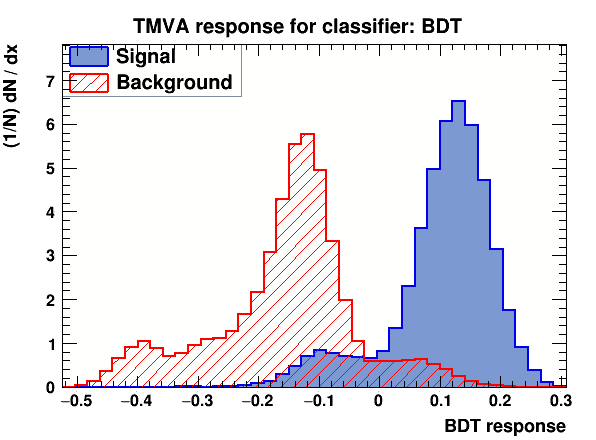
\includegraphics[width=0.48\textwidth,height=7cm,keepaspectratio]{fig/BDT}
  \caption[Classifier BDT response]{BDT response for signal and background events after TMVA classification}
  \label{Fig:BDT}
\end{figure}

\begin{figure}
  \begin{equation}
    \label{Eq:branching ratio}
    Br(H\rightarrow WW^*) = \frac{N_{BDT} - \epsilon_bL\sigma_{b}}{\epsilon_{s}N_{generated}Br(WW\rightarrow qql\nu)}
  \end{equation}
  Where ${N_{BDT}=}$ is the total number of events passing the BDT cut, ${\epsilon_a}$ \& ${\epsilon_b=}$ are the signal and background efficiency, ${L=}$ is the integrated luminosity and ${N_{generated}}$ is the total number of events in the CLIC generated samples (signal + background) 
\end{figure}

\chapter{Summary and Outlook}
  
We have discussed the physics case for future lepton colliders and demonstrated their capability for performing high precision and model independent measurements in the Higgs sector. \ac{ILC} and \ac{CLIC} have been suggested as the two main candidates for the next generation of lepton colliders. While \ac{CLIC} could argueably be described as the higher performance machine due to its greater energy range and larger luminosity, the maturity of the \ac{ILC}s project still leaves it as the more realistic choice for the next lepton collider to be built. We have also given a brief overview of the detectors and software used at each experiment to emphasize that the main design focus has been optimizing the detector for use with particle flow algorithms to improve the precision of energy measurements.

The work we have carried out so far can be split into three categories: simulation, hardware and analysis. In simulation studies we have managed to validate the performance of the \ac{ILD} electromagnetic calorimeter by generating longitudinal shower profiles and showing that ${\sim}$99.5\% of an electromagnetic particles' energy is captured by the detector. For hardware we have begun studying the use of a Digital \ac{ECAL} (in the form of Cherwell sensors) as a way to perform precise energy measurements using high granularity pixels that could help improve the performance of particle flow algoritms. So far we have managed to produce raw hitmaps for our sensors; further studies are expected to constitute a large proportion of our future work. In particluar we will be hoping to examine the performance of the sensors under power pulsing (which is currently required by the ILD detector) and when ganged together into groups of four (for use in both the tracking and calorimeter sections.) Our analysis has consisted of measuring the ${H\rightarrow WW^*}$ via the semileptonic channel. We have shown that using our reconstruction method combined with a \ac{BDT} we are capable of measuring this value to a precision of ${\sim}$5\% though this value is expected to improve significantly when we increase our statistics by using a larger background sample.

The majority of our future work will be orientated around quantifying the benefits of the Digital \ac{ECAL}. As well as performing the hardware studies mentioned above we will be doing simulation studies comparing the performance of the Digital \ac{ECAL} to the standard \ac{ECAL} design. This will be done by simulating ${e^+e^-\rightarrow HZ, Z\rightarrow\mu\bar{\mu}}$, H ${\rightarrow \tau\bar{\tau}}$ events in both versions of the detector and comparing the performance. This channel is chosen because the $\tau$ decays can produce pions that are highly clustered together making it hard for particle flow algorithms to distinguish the showers in the calorimeters as being from multiple sources. We are expecting that the high granularity of the Digital \ac{ECAL} will improve the performance by giving a higher resolution and making it easier to separate the pions showers into their different sources.
